\documentclass[a4paper]{article}

%=========================================
% Packages
%=========================================
\usepackage{mathtools}
\usepackage{amsfonts}
\usepackage{amsmath}
\usepackage{amssymb}
\usepackage{amsthm}
\usepackage[a4paper, total={6in, 8in}, margin=1in]{geometry}
\usepackage[utf8]{inputenc}
\usepackage{fancyhdr}
\usepackage[utf8]{inputenc}
\usepackage{graphicx}
\usepackage{physics}
\usepackage[listings]{tcolorbox}
\usepackage{hyperref}
\usepackage{tikz-cd}
\usepackage{adjustbox}
\usepackage{enumitem}
\usepackage[font=small,labelfont=bf]{caption}
\usepackage{subcaption}
\usepackage{wrapfig}
\usepackage{makecell}



\raggedright

\usetikzlibrary{arrows.meta}

\DeclarePairedDelimiter\ceil{\lceil}{\rceil}
\DeclarePairedDelimiter\floor{\lfloor}{\rfloor}

%=========================================
% Fonts
%=========================================
\usepackage{tgpagella}
\usepackage[T1]{fontenc}


%=========================================
% Custom Math Operators
%=========================================
\DeclareMathOperator{\adj}{adj}
\DeclareMathOperator{\im}{im}
\DeclareMathOperator{\nullity}{nullity}
\DeclareMathOperator{\sign}{sign}
\DeclareMathOperator{\dom}{dom}
\DeclareMathOperator{\lcm}{lcm}
\DeclareMathOperator{\ran}{ran}
\DeclareMathOperator{\ext}{Ext}
\DeclareMathOperator{\dist}{dist}
\DeclareMathOperator{\diam}{diam}
\DeclareMathOperator{\aut}{Aut}
\DeclareMathOperator{\inn}{Inn}
\DeclareMathOperator{\syl}{Syl}
\DeclareMathOperator{\edo}{End}
\DeclareMathOperator{\cov}{Cov}
\DeclareMathOperator{\vari}{Var}
\DeclareMathOperator{\cha}{char}
\DeclareMathOperator{\Span}{span}
\DeclareMathOperator{\ord}{ord}
\DeclareMathOperator{\res}{res}
\DeclareMathOperator{\Hom}{Hom}
\DeclareMathOperator{\Mor}{Mor}
\DeclareMathOperator{\coker}{coker}
\DeclareMathOperator{\Obj}{Obj}
\DeclareMathOperator{\id}{id}
\DeclareMathOperator{\GL}{GL}
\DeclareMathOperator*{\colim}{colim}

%=========================================
% Custom Commands (Shortcuts)
%=========================================
\newcommand{\CP}{\mathbb{CP}}
\newcommand{\GG}{\mathbb{G}}
\newcommand{\F}{\mathbb{F}}
\newcommand{\N}{\mathbb{N}}
\newcommand{\Q}{\mathbb{Q}}
\newcommand{\R}{\mathbb{R}}
\newcommand{\C}{\mathbb{C}}
\newcommand{\E}{\mathbb{E}}
\newcommand{\Prj}{\mathbb{P}}
\newcommand{\RP}{\mathbb{RP}}
\newcommand{\T}{\mathbb{T}}
\newcommand{\Z}{\mathbb{Z}}
\newcommand{\A}{\mathbb{A}}
\renewcommand{\H}{\mathbb{H}}
\newcommand{\K}{\mathbb{K}}

\newcommand{\mA}{\mathcal{A}}
\newcommand{\mB}{\mathcal{B}}
\newcommand{\mC}{\mathcal{C}}
\newcommand{\mD}{\mathcal{D}}
\newcommand{\mE}{\mathcal{E}}
\newcommand{\mF}{\mathcal{F}}
\newcommand{\mG}{\mathcal{G}}
\newcommand{\mH}{\mathcal{H}}
\newcommand{\mI}{\mathcal{I}}
\newcommand{\mJ}{\mathcal{J}}
\newcommand{\mK}{\mathcal{K}}
\newcommand{\mL}{\mathcal{L}}
\newcommand{\mM}{\mathcal{M}}
\newcommand{\mO}{\mathcal{O}}
\newcommand{\mP}{\mathcal{P}}
\newcommand{\mS}{\mathcal{S}}
\newcommand{\mT}{\mathcal{T}}
\newcommand{\mV}{\mathcal{V}}
\newcommand{\mW}{\mathcal{W}}

%=========================================
% Colours!!!
%=========================================
\definecolor{LightBlue}{HTML}{2D64A6}
\definecolor{ForestGreen}{HTML}{4BA150}
\definecolor{DarkBlue}{HTML}{000080}
\definecolor{LightPurple}{HTML}{cc99ff}
\definecolor{LightOrange}{HTML}{ffc34d}
\definecolor{Buff}{HTML}{DDAE7E}
\definecolor{Sunset}{HTML}{F2C57C}
\definecolor{Wenge}{HTML}{584B53}
\definecolor{Coolgray}{HTML}{9098CB}
\definecolor{Lavender}{HTML}{D6E3F8}
\definecolor{Glaucous}{HTML}{828BC4}
\definecolor{Mauve}{HTML}{C7A8F0}
\definecolor{Darkred}{HTML}{880808}
\definecolor{Beaver}{HTML}{9A8873}
\definecolor{UltraViolet}{HTML}{52489C}



%=========================================
% Theorem Environment
%=========================================
\tcbuselibrary{listings, theorems, breakable, skins}

\newtcbtheorem[number within = subsection]{thm}{Theorem}%
{	colback=Buff!3, 
	colframe=Buff, 
	fonttitle=\bfseries, 
	breakable, 
	enhanced jigsaw, 
	halign=left
}{thm}

\newtcbtheorem[number within=subsection, use counter from=thm]{defn}{Definition}%
{  colback=cyan!1,
    colframe=cyan!50!black,
	fonttitle=\bfseries, breakable, 
	enhanced jigsaw, 
	halign=left
}{defn}

\newtcbtheorem[number within=subsection, use counter from=thm]{axm}{Axiom}%
{	colback=red!5, 
	colframe=Darkred, 
	fonttitle=\bfseries, 
	breakable, 
	enhanced jigsaw, 
	halign=left
}{axm}

\newtcbtheorem[number within=subsection, use counter from=thm]{prp}{Proposition}%
{	colback=LightBlue!3, 
	colframe=Glaucous, 
	fonttitle=\bfseries, 
	breakable, 
	enhanced jigsaw, 
	halign=left
}{prp}

\newtcbtheorem[number within=subsection, use counter from=thm]{lmm}{Lemma}%
{	colback=LightBlue!3, 
	colframe=LightBlue!60, 
	fonttitle=\bfseries, 
	breakable, 
	enhanced jigsaw, 
	halign=left
}{lmm}

\newtcbtheorem[number within=subsection, use counter from=thm]{crl}{Corollary}%
{	colback=LightBlue!3, 
	colframe=LightBlue!60, 
	fonttitle=\bfseries, 
	breakable, 
	enhanced jigsaw, 
	halign=left
}{crl}

\newtcbtheorem[number within=subsection, use counter from=thm]{eg}{Example}%
{	colback=Beaver!5, 
	colframe=Beaver, 
	fonttitle=\bfseries, 
	breakable, 
	enhanced jigsaw, 
	halign=left
}{eg}

\newtcbtheorem[number within=subsection, use counter from=thm]{ex}{Exercise}%
{	colback=Beaver!5, 
	colframe=Beaver, 
	fonttitle=\bfseries, 
	breakable, 
	enhanced jigsaw, 
	halign=left
}{ex}

\newtcbtheorem[number within=subsection, use counter from=thm]{alg}{Algorithm}%
{	colback=UltraViolet!5, 
	colframe=UltraViolet, 
	fonttitle=\bfseries, 
	breakable, 
	enhanced jigsaw, 
	halign=left
}{alg}




%=========================================
% Hyperlinks
%=========================================
\hypersetup{
    colorlinks=true, %set true if you want colored links
    linktoc=all,     %set to all if you want both sections and subsections linked
    linkcolor=DarkBlue,  %choose some color if you want links to stand out
}

\graphicspath{ {./Images/} }

\pagestyle{fancy}
\fancyhf{}
\rhead{Labix}
\lhead{Groups and Rings}
\rfoot{\thepage}

\title{Groups and Rings}

\author{Labix}

\date{\today}
\begin{document}
\maketitle
\begin{abstract}
These notes will survey one of the most basic constructions in the entirely of algebra. Algebra had came to be from the study of symmetry, and symmetric will the definitions of a group will be. Broadly speaking abstract algebra is the study of algebraic structures. \\~\\

The first 5 chapters are dedicated to group theory , which is what happens when a set can be endowed with a binary operation that achieves some level of symmetry through inverses and identities. In particular, Lagrange's theorem and results from normal subgroups such as the first isomorphism theorem form the technical foundation of group theory, while group actions can be widely seen from all areas of mathematics. \\~\\

The remaining chapters introduces the notion of rings, which is a set with two operations instead of one, again satisfying some level of symmetry with inverses and identities. Rings form an even larger class of objects than groups, in which we classify them according to what additional properties they and the ideals of the ring has. Two important types of rings include polynomials and fields, which are themselves closely related and we will lay the foundations here and will be extensively studied and field and Galois theory. \\~\\

Famous mathematicians who contributed to this area in mathematics include Joseph Louis Lagrange, Niels Henrik Abel and Évariste Galois and, Emmy Noether, Augustin Louis Cauchy, Arthur Cayley many more. \\~\\
\textbf{References}
\begin{itemize}
\item Abstract Algebra by David S. Dummit and Richard M. Foote
\end{itemize}
\end{abstract}
\pagebreak
\tableofcontents
\pagebreak

\section{Introduction to Groups}
We begin our venture to abstract algebra with group theory. Group theorists are interested in a particular algebraic structure called a group. While they are not the simplest algebraic structure (semi groups are arguably simpler in definition), they serve as the foundation of most other algebraic structures. For example, rings, fields, vector spaces and modules can all be thought of as a group with additional structure. While semi groups and monoids are groups losing some of its constraints. 

\subsection{Basic Concepts of Groups}
We begin not by the definition of a group, but by that of a binary operation. It will serve as a central notion differentiating an ordinary set and a group. 

\begin{defn}{Binary Operation}{} A binary operation $\ast$ on a set $G$ is a function $$\ast:G\times G\to G$$
\end{defn}

Notice that the definition of a binary operation depends on both the underlying set and the definition on how the operation works on each element. To define a binary operation, one must show how any two elements of a set are combined. The new element must more over lie within the set. 

\begin{defn}{Groups}{} A group is an ordered pair $(G,\ast)$ where $G$ is a set and $\ast:G\times G\to G$ is a binary operation on $G$ satisfying the following axioms. 
\begin{itemize}
\item Associativity: $a\ast(b\ast c)=(a\ast b)\ast c$ for all $a,b,c\in G$
\item Identity element: There exists an element $e\in G$, called an identity of G, such that for all $a\in G$ we have $a\ast e=e\ast a=a$
\item Inverse element: For each $a\in G$ there is an element $a^{-1}$ of $G$, called an inverse of $a$, such that $a\ast a^{-1}=a^{-1}\ast a=e$. 
\end{itemize}
\end{defn}

We say that the above 3 defining properties the group axioms. It does feel out of place to call them axioms because they are not universal truths. To check that a set emits a group structure, we must also check that the operation defined on the set is a binary operation. This means that we actually have four axioms to check, with the fourth one being called the closure property, closure meaning that the operation on two elements lands in the same set. \\~\\

We often call the binary operation the group operation of $(G,\ast)$ to distinguish other algebraic structures on $(G,\ast)$ if it exists. Later on we often shorthand the notion of $(G,\ast)$ to just $G$, either when notation is clear or implicit. 

\begin{defn}{Abelian Groups}{} A group $(G,\ast)$ is abelian if $a\ast b=b\ast a$ for all $a,b\in G$. More generally, two elements $g,h$ in a general group $(H,\ast)$ is said to commute if $g\ast h=h\ast g$. 
\end{defn}

Simply put, it is a group where its elements are commutative with each other. Most groups that one naturally think of maybe abelian, due to the readers previously being accustomed to it. However groups that are non-abelian are also central in the study of algebraic structures. Some important examples of non-abelian groups would be the dihedral group and the symmetric group. 

\begin{prp}{}{} Let $(G,\ast)$ be a group. Then the following are true regarding the identity and inverses within $G$. 
\begin{itemize}
\item The identity of $G$ is unique
\item For each $a\in G$, $a^{-1}$ is unique
\item $(a^{-1})^{-1}=a$ for all $a\in G$
\item $(a\ast b)^{-1}=(b^{-1})\ast(a^{-1})$
\end{itemize}\tcbline
\begin{proof} Let $G$ be a group. 
\begin{itemize}
\item Let $e,f$ be identities of $G$. Let $a\in G$. Since $e$ is the identity, $ef=e$. Since $f$ is the identity, $ef=f$. Thus $e=ef=f$. 
\item Suppose that $b,c\in G$ are inverses of $a$. Since groups are associative, $(ba)c=b(ac)$. From the left, $(ba)c=ec=c$. From the right, $b(ac)=be=b$. Thus $b=(ba)c=b(ac)=c$. 
\item Suppose that $a^{-1}=b$. Since the inverse of $a$ is $b$, we have $ab=e$. But since $ab=e$, the inverse of $b$ is $a$. 
\item Suppose that the inverse of $a$ is $c$ and the inverse of $b$ is $d$. Then $(ab)(dc)=a(bd)c=ac=e$. Thus the inverse of $ab$ is $dc=b^{-1}a^{-1}$. 
\end{itemize}
\end{proof}
\end{prp}

Do be aware that since in general a group is not abelian, the inverse law above is rather important as taking the inverse also inverse the order of multiplication. It may be best to say here that we typically denote the identity as $1$. In the theory of abelian groups, the group operation will usually be denoted additively with $+$ so that the identity $0$ would make sense. However for non-abelian groups, $1$ being the identity is more common, together with the symbol of multiplication like $\cdot$ or $\times$. In these notes we will not distinguish between the two notions and we will predominantly use $1$ as the identity. Most of the time the identity should be understood through context, at least for the first few chapters on groups. \\~\\

It is also customary to write $1_G$ for the identity element of $G$ and $1_H$ for the identity element of $H$ and etc when we would like to distinguish between the identity of different groups. 

\begin{defn}{Order of an Element}{} For a group $G$ and an element $x\in G$ define the order of $x$ to be the smallest integer $n$ such that $x^n=1$, and denote this integer by $$\abs{x}=\min\{n\in\N\;|\;x^n=1\}$$ If no positive power of $x$ is the identity, the order of $x$ is defined to be infinity and $x$ is said to be of infinite order. 
\end{defn}

Aside from the order of an element, we also have the order of the entire group, which is an easier definition. 

\begin{defn}{Order of a Group}{} Let $G$ be a group. The order of $G$ is the number of elements that $G$ has, denoted by $\abs{G}$. We say that $G$ is a finite group if $\abs{G}$ is a finite number. Otherwise $G$ is an infinite group. 
\end{defn}

Both finite groups and infinite groups form an important class of groups, both of which studied extensively in different areas of abstract algebra. \\~\\

Be wary that a group does not necessarily have to contain an element of the same order of the group. However it is true that for any element $g\in G$ in a group, $\abs{g}\leq\abs{G}$. It is an easy consequence of Lagrange's theorem which we will see later. 

\begin{lmm}{}{} Let $G$ be a group. Let $k\in\N$. Then $a^k=1$ if and only if $\abs{a}$ divides $k$. \tcbline
\begin{proof}
If $k=n\abs{a}$ for some $n\in\N$ then we have $$a^k=a^{\abs{a}n}=(a^\abs{a})^n=1$$ Conversely if $a^k=1$, then since $\abs{a}$ is by definition the smallest number such that the $a^\abs{a}=1$, we can apply division algorithm to obtain $k=\abs{a}q+r$ for some $q\in\N$ and $0\leq r<n$. Now $a^{k}=a^{\abs{a}q+r}$ implies that $1=a^r$, which contradicts the minimality of $\abs{a}$. Thus we conclude. 
\end{proof}
\end{lmm}

The following theorem gives a formula for calculating the order of the power of a given element. It is exceptionally useful given that we know of the element's order. 

\begin{prp}{}{} Let $G$ be a group and $g\in G$ an element of finite order $n$. Then $$\abs{g^k}=\frac{n}{\gcd(k,n)}=\frac{\lcm(k,n)}{k}$$ for any $k\in\N$\tcbline
\begin{proof} The equality between the two expressions is trivial since $\gcd(m,n)\times\lcm(m,n)=m\times n$. Now let $b=\frac{n}{\gcd(k,n)}$ and $c=\frac{k}{\gcd(k,n)}$. Then we must have $\gcd(b,c)=1$. Now
\begin{align*}
(g^k)^b&=g^{kb}\\
&=g^{\gcd(k,n)cb}\\
&=g^{nc}\\
&=(g^n)^c\\
&=1
\end{align*}
Thus we must have $\abs{g^k}$ divides $\frac{n}{\gcd(k,n)}$. Now we know that $g^{k\abs{g^k}}=(g^k)^{\abs{g^k}}=1$. Thus we must have $n$ divides $k\abs{g^k}$, meaning $\gcd(k,n)b$ divides $\gcd(k,n)c\abs{g^k}$ and $b$ divides $c\abs{g^k}$. We know that $\gcd(b,c)=1$ thus $b$ divides $\abs{g^k}$. From the fact that $b=\frac{n}{\gcd(k,n)}$ we have $\abs{g^k}$ divides $b$ as well and thus $b=\abs{g^k}$ and $$\abs{g^k}=\frac{n}{\gcd(k,n)}$$
\end{proof}
\end{prp}

In general finding the order of the product of elements is a hard problem. In the case that two elements commute, the order of their product is somehow determined by their individual orders, which makes it easier to deduce. 

\begin{lmm}{}{} Let $G$ be a group. Let $a,b\in G$ be elements that commute with each other. Then $\abs{ab}$ divides $\lcm(\abs{a},\abs{b})$. \tcbline
\begin{proof}
Let $l=\lcm(\abs{a},\abs{b})$. Since $a$ and $b$ commutes, we have that $$(ab)^l=a^lb^l=1$$ and so $\abs{ab}$ divides $l$. 
\end{proof}
\end{lmm}

We will see in the section of cyclic groups that we can impose a stronger condition so that the above result is an equality. 

\subsection{Subgroups}
The idea of a subgroup is that some (not all) elements in a group can also form a group in and of itself. Most of the structure of a group carries on to its subgroup, while the converse may not necessarily be true. 

\begin{defn}{Subgroups}{} If $(G,\ast)$ is a group and $H$ is a subset of $G$ such that $(H,\ast)$ is a group $(H,\ast)$. Then $H$ is called a subgroup of $G$ and is denoted $H\leq G$. 
\end{defn}

Subgroups are still part of the larger group. This means that if $H$ is a subgroup of $G$, then certain properties of $H$ are inherited from $G$. For example, the uniqueness of the identity element ensures that $H$ and $G$ share the same identity element. 

\begin{lmm}{}{} Let $G$ be a group and $H\leq G$. Then $1_H=1_G$. \tcbline
\begin{proof}
If $1_H\neq 1_G$ then there will be two identities in $G$. 
\end{proof}
\end{lmm}

To check that a subset of a group is a subgroup, it is not necessary to go through the four axioms of a group as it is rather tedious. Instead, we may turn to an easier criterion which involves less work. 

\begin{thm}{Criterion for a Subgroup}{} Let $(G,\ast)$ be a group. A subset $H$ of $G$ is a subgroup if and only if 
\begin{itemize}
\item If $a,b\in H$ then $a\ast b\in H$
\item If $a\in H$ then $a^{-1}\in H$
\end{itemize}\tcbline
\begin{proof} We first prove the forward implication. Suppose that $H$ is a subgroup. Then by definition of a group the above are all true.\\~\\
Suppose that $H$ is satisfies the above two conditions. We show that it implies the four definitions of a group. Since $a,b\in H$ implies $ab\in H$, closure is satisfied. Since $H\subseteq G$, and $G$ is associative, $H$ is also associative. If $a\in H$ then $a^{-1}\in H$ thus inverse exists. Finally since $H$ is closed, $aa^{-1}=1\in H$ thus identity is in $H$. Thus $H$ is a group. 
\end{proof}
\end{thm}

We thern have subgroups that exists within every group. They are called trivial since we usually do not want to deal with them. 

\begin{lmm}{Trivial Subgroups}{} Let $G$ be a group. Then $G$ and $\{1\}$ are subgroups of $G$. \tcbline
\begin{proof} Both can easily be seen to satisfy the subgroup criterion. 
\end{proof}
\end{lmm}

The final proposition gives a new way of generating a subgroup given two subgroups. In particular, their overlapping part is also a subgroup in itself. 

\begin{prp}{}{} Let $G$ be a group and $H,K$ subgroups of $G$. Then $H\cap K$ is a subgroup of $G$. \tcbline
\begin{proof} Suppose that $H,K$ are subgroups of $G$. We show that $H\cap K$ with the subgroup criterion. We have that 
\begin{itemize}
\item $1\in H$ and $1\in K$ thus $1\in H\cap K$
\item Suppose that $a,b\in H\cap K$. Then since $ab\in H$ and $ab\in K$ we have $ab\in H\cap K$
\item Suppose that $a\in H\cap K$ since $H$ and $K$ are subgroups respectively, $a^{-1}\in H$ and $a^{-1}\in K$ thus $a^{-1}\in H\cap K$. 
\end{itemize}
The subgroup criterion is satisfied thus $H\cap K$ is a subgroup of $G$. 
\end{proof}
\end{prp}

\subsection{Generators of a Group}
Cyclic groups appear in a lot of diverse areas of mathematics such as topology and number theory. It structure is simple enough to be employed in different areas while the notions it encapsulates is broad. 

\begin{defn}{Cyclic Subgroups}{} Let $G$ be a group. Define $$\langle g\rangle=\{g^k|k\in\Z\}$$ to be the cyclic subgroup generated by $g$. In this case, $g$ is the generator of $\langle g\rangle$. \\~\\
A group $G$ is called cyclic if there exists some $g\in G$ such that $G=\langle g\rangle$. 
\end{defn}

Cyclic subgroups arise in the simplest context in any group. The following proposition demonstrates that every group contains a cyclic subgroup. 

\begin{prp}{}{} Let $G$ be a group and $g\in G$. Then $\langle g\rangle$ is a subgroup of $G$. \tcbline
\begin{proof} We prove that it satifies the subgroup criterion. 
\begin{itemize}
\item $g^0=1$ thus $1\in\langle g\rangle$ 
\item $g^{-1}$ is in $\langle G\rangle$ is trivial
\item Let $a,b\in\langle g\rangle$. Then $a=g^n$ and $b=g^m$ for some $n,m\in\Z$ thus $ab=g^{n+m}\in\langle g\rangle$. 
\end{itemize}
The subgroup criterion is satisfied thus we are done. 
\end{proof}
\end{prp}

In particular, the cyclic subgroup of a group $G$ can be constructed simply by taking any one element in $G$ and consider all the powers (positive and negative) of the element. \\~\\

it is easy to see that cyclic groups commute through their power. 

\begin{lmm}{}{} Cyclic groups are abelian. \tcbline
\begin{proof}
Let $\langle g\rangle$ be a cyclic group. Then for any $g^m,g^n\in\langle g\rangle$, we have that $$g^m\cdot g^n=g^{m+n}=g^{n+m}=g^n\cdot g^m$$ and so we conclude. 
\end{proof}
\end{lmm}

The following result would seem quite trivial at first sight. It makes sense to think that a subgroup of a cyclic group would be cyclic. The proof however does not look trivial at all. It is one of the first proofs that uses some notion in number theory, showing some linkage between the two subjects. 

\begin{prp}{}{} Let $G=\langle g\rangle $ be a cyclic group. Then any subgroup $H$ of $G$ is also cyclic. \tcbline
\begin{proof} Let $H\leq G=\langle g\rangle$. Every element in $H$ is of the form $g^n$ for some $n\in\Z$. Take the smallest positive $k$ such that $g^k\in H$. Consider another element $g^n\in H$. By the division algorithm, $n=qk+r$ for some $r\in\{0,\dots,k-1\}$. Thus we have $$g^n=g^{kq+r}\iff g^r=(g^k)^{-q}(g^n)$$ Now since $g^k\in H$, $(g^k)^{-1}\in H$ and $(g^k)^q\in H$ thus $(g^k)^q\in H$ and $(g^k)^q(g^n)\in H$ by inverse and closure of a group. Thus $g^r\in H$. However this is a contradiction since $k$ is the least power of $g$ such that $g^k\in H$ but $g^r$ with $r<k$ is now in $H$. Thus we must have $r=0$ and $g^n=(g^k)^q$. This applies for every $g^n\in H$ thus $H=\langle g^k\rangle$. 
\end{proof}
\end{prp}

One can also show that in the case of a cyclic group, the order of the group is equal to the order of the generator. However the converse is not always true. That is, the order of the group and the order of one particular element being the same does not imply that the group is cyclic. 

\begin{prp}{}{} Suppose that $G=\langle g\rangle $. Then $\abs{G}=\abs{g}$. \tcbline
\begin{proof} Suppose that $\abs{g}=n$ Note that $g^{n+k}=g^k$ for any $k\in\{0,\dots,n-1\}$. Thus $\{g^n|n\in\mathbb{Z}\}$ has $n$ distinct elements. Thus $\abs{G}=n$. \\~\\
If $\abs{g}=\infty$ then $g^n\neq 1$ for all $n$ not equal to $0$. Thus $\{g^n|n\in\mathbb{Z}\}$ are all distinct and $\abs{G}=\infty$.
\end{proof}
\end{prp}

Using cyclic subgroups, we can impose a stronger condition so that the order of the product of two elements can be given an explicit formula. 

\begin{prp}{}{} Let $G$ be a group and $a,b\in G$ such that $a,b$ commutes. If furthermore $\langle a\rangle\cap\langle b\rangle=\{1\}$, then $$\abs{ab}=\lcm(\abs{a},\abs{b})$$ \tcbline
\begin{proof}
Let $n=\abs{ab}$. Since $a$ and $b$ commute, we have that $$1=(ab)^n=a^nb^n$$ so that $a^n=b^{-n}$. Thus $a^n\in\langle b\rangle$. But $a^n\in\langle a\rangle\cap\langle b\rangle=\{1\}$ implies that $a^n=1$. Similarly, we have that $b^n=1$. This means that we have $\abs{a},\abs{b}$ divides $n$. and thus $\lcm(\abs{a},\abs{b})$. We know from groups and rings that $\abs{ab}$ divides $\lcm(\abs{a},\abs{b})$ and so we conclude. 
\end{proof}
\end{prp}

\subsection{Homomorphisms and Isomorphisms}
Homomorphisms and isomorphisms are important concepts not only in terms of the ability to classify groups with similar structure, but is also useful in the creation of new groups, such as subgroups and quotient groups. One common idea throughout all of mathematics is to not only study the object itself, but to also study functions in and out of the object. In the case of groups, a meaningful function would be one that preserve the study of a group. This leads to the definition of a group homomorphism. 

\begin{defn}{Group Homomorphisms}{} Let $(G,*)$ and $(H,\circ)$ be groups. A map $\phi:G\to H$ such that $$\phi(x*y)=\phi(x)\circ\phi(y)$$ for all $x,y\in G$ is called a homomorphism. 
\end{defn}

As a result of preserving group structures, group homomorphisms are way more rigid compared to a regular function. In particular, all of the following are true regarding an arbitrary group homomorphism. 

\begin{prp}{}{} Let $\phi:G_1\to G_2$ be a group homomorphism. Then the following are true regarding $\phi$. 
\begin{itemize}
\item $\phi(1)=1$
\item $\phi(g^{-1})=\phi(g)^{-1}$ for all $g\in G_1$
\item $\phi(g^n)=\phi(g)^n$ for all $n\in\mathbb{N}$ and all $g\in G_1$
\end{itemize}\tcbline
\begin{proof} Let $\phi:G\to H$ be a homomorphism. 
\begin{itemize}
\item We have that 
\begin{align*}
\phi(1)&=\phi(1\cdot 1)\\
\phi(1)&=\phi(1)\cdot\phi(1)\\
\phi(1)\phi(1)^{-1}&=\phi(1)\phi(1)\phi(1)^{-1}\\
1&=\phi(1)
\end{align*}
\item We have that $$\phi(g)\phi(g^{-1})=\phi(gg^{-1})=\phi(1)=1$$ and $$\phi(g)\phi(g)^{-1}=1$$ Also since the inverse is unique, we have that $\phi(g^{-1})=\phi(g)^{-1}$
\item We have that $\phi(g)\cdots\phi(g)=\phi(g\cdots g)$ by applying the definition of homomorphism $n-1$ times
\end{itemize}
And so we conclude. 
\end{proof}
\end{prp}

Structures that can be seen carrying over would be power, inverses, subgroups and identities. But these are only some of the capabilities of a homomorphism. 

\begin{defn}{Kernel}{} Let $\phi:G\to H$ be a homomorphism. Define the kernel of $\phi$ to be $$\ker(\phi)=\{g\in G|\ker(g)=1_H\}$$
\end{defn}

This notion is exactly parallel to that of linear algebra. They are both the kernel in the sense that they are the element that maps to the identity. In fact, as readers will see in module theory, the entire theory of linear algebra is simply a special case of module theory. 

\begin{prp}{}{} Let $\phi:G\to H$ be a homomorphism. Then $\ker(\phi)$ is a subgroup of $G$. \tcbline
\begin{proof}
We prove closure, identity and inverse as stated by the subgroup criterion. 
\begin{itemize}
\item $\phi(1_G)=1_H$, thus we have $1_G\in\ker(\phi)$
\item If $a,b\in\ker(\phi)$, then $\phi(a)=1$ and $\phi(b)=1$ and $$\phi(ab)=\phi(a)\phi(b)=1$$ thus $ab\in\ker(\phi)$. 
\item If $a\in\ker(\phi)$ then $$1=\phi(1)=\phi(aa^{-1})=\phi(a)\phi(a^{-1})=\phi(a^{-1})$$ By the subgroup criterion $\ker(\phi)\leq G$. 
\end{itemize}
\end{proof}
\end{prp}

When a map of sets have an inverse, we say that the two sets are bijective. When a group homomorphisms has an inverse, we have the corresponding notion called isomorphic. 

\begin{defn}{Group Isomorphisms}{} Let $G,H$ be groups. A map $\phi:G\to H$ is said to be an isomorphism if $\phi$ is a bijective homomorphism. In this case we say that $G\cong H$ and that $G$ and $H$ are isomorphic groups. 
\end{defn}

Isomorphisms are stricter in the sense that the structure between the two groups it reflects has a higher compatibility than that of homomorphism. 

\begin{prp}{Properties of Isomorphism}{} Let $G,H$ be groups. If a map $\phi:G\to H$ is isomorphic, then
\begin{itemize}
\item $\phi^{-1}$ is an isomorphism
\item $\abs{G}=\abs{H}$
\item $\ker(\phi)=\{1\}$
\item $G$ is abelian if and only if $H$ is abelian
\item $G$ is cyclic if and only if $H$ is cyclic
\item $\abs{x}=\abs{\phi(x)}$
\item $G$ has a subgroup of order $k$ if and only if $H$ has a subgroup of order $k$. 
\end{itemize}\tcbline
\begin{proof} Suppose that $\phi$ is a bijection of $G$ and $H$. 
\begin{itemize}
\item Since $\phi$ is bijective, $\phi^{-1}$ is also bijective thus it is well defined. But we also need to prove that $\phi^{-1}$ is a homomorphism. Let $h_1,h_2\in H$. Then there exists unique $g_1,g_2\in G$ such that $\phi(g_1)=h_1$ and $\phi(g_2)=h_2$. Then $$\phi^{-1}(h_1h_2)=\phi^{-1}(\phi(g_1)\phi(g_2))=\phi^{-1}(\phi(g_1g_2))=g_1g_2=\phi^{-1}(h_1)\phi^{-1}(h_2)$$ thus we are done. 
\item Since $\phi$ is bijective, $\abs{G}=\abs{H}$
\item Since $\phi$ is bijective and $1\in\ker(\phi)$, we must have $\ker(\phi)=\{1\}$
\item Suppose that $G$ is abelian. $\phi(a)\phi(b)=\phi(ab)=\phi(ba)=\phi(b)\phi(a)$. Thus $H$ is abelian. Since $\phi$ is bijective it has a bijective inverse. Thus the backwards implication is proved. 
\item Suppose that $x\in G$ has order $n$. $1_H=\phi(1_G)=\phi(x^n)=\phi(x)^n$
\item If $\abs{x}=n$ then $\phi(x)^n=\phi(x^n)=\phi(1)=1$ thus we know that $\abs{\phi(x)}\bigg{|}n$. However for any $k<n$, $\phi(x)^k=\phi(x^k)\neq 1$ since $\phi$ is an isomorphism and $\ker(\phi)=\{1\}$. Thus we must have $\abs{\phi(x)^n}=1$. 
\item Suppose that $G$ has a subgroup of order $k$, then $\phi(G)$ is a subgroup as well and every element preserves its order, we have that $\phi(G)\leq H$ is order $k$. For the reverse statement, just take $\phi^{-1}$ to be the isomorphism. 
\end{itemize}
And so we conclude. 
\end{proof}
\end{prp}

Isomorphisms capture more sturcture than homomorphism such as orders, commutativity, subgroups of particular orders and whether the group is cyclic. Most of the classification results require groups to be identified up to isomorphism. \\~\\
To provide more examples of group, we can construct the automorphism group from a group. 

\begin{defn}{The Automorphism Group}{} Let $G$ be a group. An automorphism of $G$ is a group homomorphism $\phi:G\to G$. Define the automorphism group $G$ to be $$\text{Aut}(G)=\{\phi:G\to G\;|\;\phi\text{ is an isomorphism }\}$$
\end{defn}

\begin{lmm}{}{} Let $G$ be a group. Then the automorphism group $\text{Aut}(G)$ is indeed a group. \tcbline
\begin{proof}
Composing bijective maps also gives bijective maps and so composition is a binary operation. This operation is associative since composition of functions is associative. The identity map $\text{id}_G$ of $G$ is the identity of the automorphism group since for any automorphism $\phi:G\to G$, we have that $$\phi\circ\text{id}_G=\phi=\text{id}_G\circ\phi$$ Finally, each automorphism is a bijection and so is invertible. The inverse of an automorphism is again an automorphism and so we conclude. 
\end{proof}
\end{lmm}

We will see it reappear later on when inner automorphisms is defined. For now, treat it as another example for you to work on as a group. 

\subsection{The Cyclic Groups}
The collection of all cyclic groups is one of the many classes of groups that serves as the equivalent of primes in the collection of all groups. These groups are called finite simple groups. 

\begin{defn}{The Cyclic Group $C_n$}{} Let $n\in\N$. The cyclic group of order $n$ is defined to be the group $$C_n=\{1,g,g^2,\dots,g^{n-1}\}=\langle g\rangle$$ where multiplication is defined by $g^m\cdot g^k=g^{m+k}$. It may also be denoted as $Z_n$
\end{defn}

This class of groups form an infinite family since two cyclic groups are isomorphic if and only if they have the same order. However, there may be more than $1$ generators for the group, all of which are demonstrated in the following theorem. 

\begin{thm}{}{} Let $n\in\N$ and $0\leq k\leq n-1$ be an integer. Then $g^k$ is a generator of $C_n$ if and only if $\gcd(k,n)=1$. \tcbline
\begin{proof}
Suppose that $g^k$ is a generator of $C_n$. Then $g=g^{ak}$ for some $a\in\Z$. Since $g^n=1$, there exists $b\in\Z$ such that $g^{ak-bn}=g$ and $0\leq ak-bn\leq n-1$. Then $ak-bn=1$ has a solution if and only if $\gcd(k,n)=1$ thus we are done. \\~\\
Now suppose that $\gcd(k,n)=1$. Then $\abs{g^k}=\frac{n}{\gcd(k,n)=n}$ thus we are done. 
\end{proof}
\end{thm}

\pagebreak
\section{Cosets and Quotient Groups}
\subsection{Cosets}
\begin{defn}{Cosets}{} Let $H$ be a subgroup of $G$. Let $g\in G$. 
\begin{itemize}
\item $gH=\{gh|h\in H\}$ the left cosets of $H$ generated by $H$
\item $Hg=\{hg|h\in H\}$ the right cosets of $H$ generated by $H$
\end{itemize}
\end{defn}

\begin{prp}{}{} Let $H$ be a subgroup of $G$ and let $g_1,g_2\in G$. Then the following are equivalent. 
\begin{itemize}
\item $g_1H=g_2H$
\item $g_2\in g_1H$
\item $g_1^{-1}g_2\in H$
\end{itemize}\tcbline
\begin{proof} Let $H\leq G$. 
\begin{itemize}
\item $(1)\implies(2)$ Suppose that $g_1H=g_2H$. Let $g_1h\in g_1H$. Then there exists $k$ such that $g_1h=g_2k$. Then $g_2=g_1hk^{-1}$ and since $H$ is a subgroup, $hk^{-1}\in H$ and thus $g_2\in g_1H$
\item $(1)\implies(3)$ Similar to the above argument but we rewrite the expression as $g_1^{-1}g_2=hk^{-1}$ thus $g_1^{-1}g_2\in H$
\item $(3)\implies(1)$ Let $g_2h\in g_2H$. By $(3)$ there exists $k\in H$ such that $g_1^{-1}g_2=k$. We then have 
\begin{align*}
g_1^{-1}g_2&=k\\
g_1^{-1}g_2h&=kh\\
g_2h&=g_1kh\\
g_2h&\in g_1H
\end{align*} Since $kh\in H$. Thus $g_2H\subseteq g_1H$. Mirror the argument for $g_2^{-1}g_1\in H$ and we have that $g_1H\subseteq g_2H$ and we are done
\end{itemize}
\end{proof}
\end{prp}

\begin{prp}{}{} Let $H$ be a subgroup of $G$. Let $g_1,g_2\in G$. Then $g_1H=g_2H$ if and only if $Hg_1=Hg_2$. \tcbline
\begin{proof} Let $g_1H=g_2H$. Let $hg_1\in Hg_1$. Since we know that $g_1g_2^{-1}\in H$, then $hg_1g_2^{-1}\in H$. Let $hg_1g_2^{-1}=k\in H$. Then $hg_1=kg_2\in Hg_2$ thus we have that $Hg_1\subseteq Hg_2$. The argument is similar for $Hg_2\subseteq Hg_1$ thus we have that $Hg_1=Hg_2$. For the reverse, the argument is also similar. 
\end{proof}
\end{prp}

\begin{prp}{}{} Let $H$ be a subgroup of $G$. Then the left (right) cosets of $G$ partition $G$. \tcbline
\begin{proof} We first show that if $g_1H\neq g_2H$, then $g_1H\cap g_2H=\emptyset$. Suppose that $k\in g_1H\cap g_2H$, then by the above we have $g_1H=kH=g_2H$ thus a contradiction. Thus we must have $g_1H\cap g_2H=\emptyset$. Now we must have that $$\bigcup_{g\in G}gH=G$$ since every $gH$ must at least have $g\in gH$. Thus   we are done. 
\end{proof}
\end{prp}

\begin{prp}{}{} Let $H$ be a subgroup of $G$. Then the number of distinct left cosets is equal to the number of distinct right cosets. \tcbline
\begin{proof} Since all the distinct left cosets partition $G$ and $g_1H=g_2H$ if and only if $Hg_1=Hg_2$, we must have the same number of distinct right cosets as well in order to partition $G$. 
\end{proof}
\end{prp}

\begin{prp}{}{} Let $H$ be a subgroup of a finite group $G$. Then for any $g\in G$, $\abs{gH}=\abs{H}$. \tcbline
\begin{proof} Let $g\in G$. We prove that the map $\phi:H\to gH$ defined by $\phi(h)=gh$ is a bijection. For injectivity, $gh_1=gh_2$ implies $h_1=h_2$ by applying $g^{-1}$ on both sides. Let $k\in gH$, then there exists $h\in H$ such that $k=gh\in gH$. This proves surjectivity and we are done. 
\end{proof}
\end{prp}

\begin{defn}{Number of Distinct Cosets}{} Let $H$ be a subgroup of $G$. Define $[G:H]$ to be the number of distinct left cosets of $H$ in $G$. 
\end{defn}

The set of all left (right) cosets is also important for the construction of quotient groups as well as one of the major players in group actions. 

\begin{defn}{Set of Cosets}{} Let $G$ be a group and $H$ a subgroup. Define $$\frac{G}{H}=\{gH\;|\;g\in G\}$$ the set of cosets of $H$ in $G$. 
\end{defn}

\subsection{Lagrange's Theorem}
Lagrange's theorem is a powerful theorem that has many applications. Some indirect results include the class equation and orbit stabilizer theorem as we will later see. 

\begin{thm}{Lagrange's Theorem}{} Let $G$ be a finite group and $H$ a subgroup of $G$. Then $$\abs{G}=[G:H]\abs{H}$$ \tcbline
\begin{proof} We know that distinct left cosets partition $G$ and every left coset has $\abs{H}$ elements thus $\abs{G}=[G:H]\abs{H}$. 
\end{proof}
\end{thm}

An immediate result is that orders of subgroups must divide the order of the group. Notice that this does not imply the converse: given any number $n$ that divides the order of $G$, it does not necessarily mean that there exists a subgroup of $G$ with order $n$. As always, it is good to think of counterexamples. A prototypical one would be $A_4$ (see chapter 5 for definition) that does not have subgroups of order $6$. This is the smallest example. \\~\\

Another immediate result of Lagrange's theorem is the following. 

\begin{crl}{}{} Let $G$ be a finite group and $g\in G$. Then the order of $g$ divides the order of $G$. \tcbline
\begin{proof} For every $g\in G$, $\langle g\rangle\leq G$ thus by Lagrange's Theorem $\abs{g}=\abs{\langle g\rangle}\bigg{|}\abs{G}$
\end{proof}
\end{crl}

\begin{crl}{}{} Let $G$ be a group of prime order $p$. Then $G$ is cyclic. \tcbline
\begin{proof}
For any $1\neq g\in G$, $\langle g\rangle$ is a subgroup of $G$. By Lagrange's theorem, it must divide the order of $G$, which is $p$. Since $p$ is a prime, we must have $\langle g\rangle=G$. 
\end{proof}
\end{crl}

\subsection{Normal Subgroups}
Given we have defined the set of cosets $\frac{G}{H}$ for a group $G$ and a subgroup $H$, it is normal to ask in what situations will $\frac{G}{H}$ be a group in its own right. The answer to this is completely characterized by the notion of normal subgroups. 

\begin{defn}{Normal Subgroups}{} Let $N$ be a subgroup of $G$. $N$ is called a normal subgroup of $G$ if $gN=Ng$ for all $g\in G$. We write $N\trianglelefteq G$ in this case. 
\end{defn}

\begin{defn}{Conjugates}{} Let $H$ be a subgroup of $G$. The set $$gHg^{-1}=\{ghg^{-1}|h\in H\}$$ is called the conjugate of $H$. 
\end{defn}

It does not need deep results to see that conjugations and normal subgroups are related notions. 

\begin{thm}{Normality Test}{} Let $N$ be a subgroup of $G$. The following are equivalent. 
\begin{itemize}
\item $N$ is normal in $G$
\item $gNg^{-1}\subseteq N$ for all $g\in G$
\item $gNg^{-1}=N$ for all $g\in G$
\end{itemize}\tcbline
\begin{proof} Let $N\trianglelefteq G$. 
\begin{itemize}
\item $(1)\implies(2)$ Let $N$ be normal. Let $gng^{-1}\in gNg^{-1}$. Since $N$ is normal there exists $k\in N$ such that $gn=kg$. Then $gng^{-1}=kgg^{-1}=k\in N$. 
\item $(2)\implies(1)$ Let $gNg^{-1}\subseteq N$. Then for all $n\in N$ there exists $k\in N$ such that $gng^{-1}=k$. Then $gn=kg$ for all $n$ thus $gN=Ng$ and we are done. 
\item $(2)\implies(3)$ We only need to show that $N\subseteq gNg^{-1}$. Let $n\in N$. Then $ng\in Ng$. Since $N$ is normal, there exists $k\in N$ such that $gk=ng$ and $k=g^{-1}ng$. But then $n=gkg^{-1}$ thus $n\in gNg$ and we are done. 
\item $(3)\implies(2)$ is trivial. 
\end{itemize}
\end{proof}
\end{thm}

While the second item above is simply for ease of proving things, the important thing to take away here is that as long as conjugating results in the same group, that group would be normal. 

\begin{thm}{}{} Let $H$ be a subgroup of a group $G$. Write $g_1H\cdot g_2H=\{ab|a\in g_1H,b\in g_2H\}$. Then $$g_1H\cdot g_2H=(g_1g_2)H$$ for all $g_1,g_2\in G$ if and only if $H\trianglelefteq G$. \tcbline
\begin{proof}
Suppose first that $g_1H\cdot g_2H=(g_1g_2)H$. Let $g\in G$. We want to show that $gHg^{-1}\subseteq H$. Notice that $gH\cdot g^{-1}H=H$. For any $h\in H$, we have $gh\in gH$ and $g^{-1}\in g^{-1}H$ so that $ghg^{-1}\in G$. \\~\\

Now suppose that $N$ is normal. Let $g_1h_1\in g_1H$ and $g_2h_2\in g_2H$. Then we have $$g_1h_1g_2h_2=g_1g_2h_3h_2\in(g_1g_2)H$$ since $N$ is normal and $h_1g_2=g_2h_3$. Thus $g_1H\cdot g_2H\subseteq(g_1g_2)H$. Now suppose that $g_1g_2h\in(g_1g_2)H$. Then in particular this element lies in $g_1H\cdot g_2 H$ because $g_1g_2h=g_1\cdot 1\cdot g_2\cdot h$. And so we conclude. 
\end{proof}
\end{thm}

This theorem shows that if $N$ is a normal subgroup, then the above operation is a binary operation on $G/N$. The rest of the conditions to check that $G/N$ forms a group is fairly straight forward. 

\begin{prp}{}{} Let $G$ be a group and $N$ a normal subgroup of $G$. Then $G/N$ together with the binary operation $\cdot:G/N\times G/N\to G/N$ defined by $$(gN)\cdot(hN)=(gh)N$$ is a group. \tcbline
\begin{proof}
We check the group axioms: 
\begin{itemize}
\item Associativity: Let $gN$, $hN$ and $kN$ be in $G/N$. Then by two applications of the above theorem, we have that $((gN)\cdot(hN))\cdot(kN)=(ghN)\cdot(kN)=(gh)kN$ By associativity of $G$, we conclude. 
\item Identity: Let $gN\in G/N$. Then it is clear that $(gN)\cdot(N)=(g\cdot 1)N=gN$ so that $N$ is the identity in $G/N$. 
\item Inverse: Let $gN\in G/N$. Then we can see that $(gN)\cdot(g^{-1}N)=(gg^{-1})N=N$ so that each element in $G/N$ has an inverse. 
\end{itemize}
All the group axioms are satisfied and so we conclude. 
\end{proof}
\end{prp}

\begin{defn}{Quotient Group}{} Let $G$ be a group and $N$ a normal subgroup of $G$. Define the quotient group of $G$ with $N$ to be the group $G/N$. 
\end{defn}

Normal subgroups are also closely related to kernels. This is because for any group $G$ and normal subgroup $N$, there is a canonical projection map $p:G\to G/N$. 

\begin{prp}{}{} A subgroup $N$ of the group $G$ is normal if and only if it is the kernel of some homomorphism. \tcbline
\begin{proof}
Suppose that $N$ is a normal subgroup of $G$. Then consider the homomorphism $\phi:G\to G/N$ defined by $\phi(g)=gN$. Then
\begin{align*}
\ker(\phi)&=\{g\in G|\phi(g)=N\}\\
&=\{g\in G|gN=N\}\\
&=\{g\in G|g\in N\}\\
&=N
\end{align*} Thus we are done. \\~\\

Let $N$ be the kernel of the homomorphism $\phi:G\to H$. Then $\ker(\phi)=\{g\in G|\phi(g)=1\}=N$. By the normality test, showing that $gng^{-1}\in N$ is sufficient for $n\in N$ and $g\in G$. We have that $$\phi(gng^{-1})=\phi(g)\phi(n)\phi(g^{-1})=\phi(g)\phi(g)^{-1}=1$$ thus $gng^{-1}\in\ker(\phi)=N$ thus we are done. 
\end{proof}
\end{prp}

Undoubtedly aside from the construction of the quotient group, the above proposition is the main result of this section. It is equivalent to say that a normal subgroup is exactly the kernel of some homomorphism. 

\subsection{Normalizers}
Sometimes, not every element in a group allows a subgroup $H$ to normalize. Therefore can obtain a subset of $G$ that  contains all the elements that allows $H$ to be normal. 

\begin{defn}{Normalizers}{} Let $G$ be a group. Let $S\subseteq G$. Then the normalizer is defined to be $$N_G(S)=\{g\in G\;|\;gS=Sg\}=\{g\in G\;|\;gSg^{-1}=S\}$$
\end{defn}

\begin{prp}{}{} Let $G$ be a group and $S\subseteq G$. Then $S\subseteq N_G(S)\leq G$. \tcbline
\begin{proof}
Let $g,h\in N_G(S)$. Then $h^{-1}\in N_G(S)$ since $h^{-1}S=Sh^{-1}$ if and only if $hS=Sh$ thus $h^{-1}\in N_G(S)$. Now we want $gh^{-1}\in N_G(S)$. We have $$gh^{-1}S=g(Sh^{-1})=(gS)h^{-1}=Sgh^{-1}$$ and so we have that $N_G(S)\leq G$. For the remaining part, if $s\in S$, then $sS=S=Ss$ and so $S\subseteq N_G(S)$. 
\end{proof}
\end{prp}

\begin{prp}{}{} Let $G$ be a group and $H$ a subgroup of $G$. Then we have $H\trianglelefteq N_G(H)$. \tcbline
\begin{proof}
We know that $H\subseteq N_G(H)$. Since $H$ and $N_G(H)$ are both subgroups of $G$, we must have $H\leq N_G(H)$. By definition of $N_G(H)$, if $g\in N_G(H)$ then $gHg^{-1}=H$ and so we conclude. 
\end{proof}
\end{prp}

\begin{prp}{}{} Let $G$ be a group and $N\subseteq G$. Then $N\trianglelefteq G$ if and only if $N_G(N)=G$. \tcbline
\begin{proof}
Let $N\trianglelefteq G$. Trivially we already have $N_G(N)\leq G$. Let $g\in G$. Then since $N$ is normal, we have $gN=Ng$ thus $g\in N_G(N)$ and we are done. \\~\\
Let $N_G(N)=G$. Then for all $g\in G$, $gN=Ng$ thus $N$ is normal. 
\end{proof}
\end{prp}

As motivated from above, $N_G(S)$ is just all the elements in $G$ so that $S$ is allowed to be normal. Then obviously if $N_G(S)$ is the entirety of $G$ then $S$ would be allowed to be normal. 

\subsection{The Isomorphism Theorems for Groups}
\begin{thm}{The First Isomorphism Theorem}{} Let $\phi:G\to H$ be a homomorphism. Then the following are true regarding the kernel and the image of the homomorphism. 
\begin{itemize}
\item $\ker(\phi)\trianglelefteq G$
\item $\im(\phi)\leq H$
\end{itemize} 
Moreover we have that $$\frac{G}{\ker(\phi)}\cong\phi(G)$$ \tcbline
\begin{proof}
Proposition 2.3.7 shows that $\ker(\phi)$ is a normal subgroup of $G$. \\~\\

Let $\phi(g),\phi(h)\in\im(\phi)$. Then $\phi(g)\cdot\phi(h)=\phi(gh)\in\im(\phi)$ so that closure is satisfied. Now clearly $\phi(g)^{-1}\in\im(\phi)$ since $\phi(g^{-1})=\phi(g)$ and so we conclude. \\~\\

We construct an isomorphism $f$ between cosets of $G$ of $\ker(phi)$ and elements of $\phi(G)$. Write $N$ for $\ker(\phi)$ Let $gN\in G/\ker(\phi)$. Define $f$ by $f(gN)=\phi(g)$. I claim that this is the isomorphism we need. \\~\\
We first show that this map is well defined. The point here is to show that any representative is fine. In particular, if $gH=hN$ are two representations of $the same coset$ and $g,h$ is distinct, then we want $f(gN)=f(hN)$. Well $gN=hN$ if and only if $gh^{-1}\in N$. This means that $gh^{-1}\in\ker(\phi)$ and $\phi(gh)^{-1}=1$. This means that $\phi(g)\phi(h)^{-1}=1$ and $\phi(g)=\phi(h)$. This means that the map is well defined. \\~\\
We now show that it is a homomorphism. Let $gN$ and $hN$ be cosets. Then $$f((gN)(hN))=f((gh)N)=\phi(gh)=\phi(g)\phi(h)=f(gN)f(hN)$$ thus we are done. Finally we show that it is an isomorphism. Firstly let $f(gN)=f(hN)$. Then
\begin{align*}
f(gN)&=f(hN)\\
\phi(g)&=\phi(h)\\
\phi(g)\phi(h)^{-1}&=1\\
\phi(gh^{-1})&=1
\end{align*}
This means that $gh^{-1}\in\ker(\phi)$ thus $gN=hN$. Now let $\phi(g)\in\phi(G)$. Then quite obviously $f(gN)=\phi(g)$ thus it is surjective and bijective and we are done. 
\end{proof}
\end{thm}

The first isomorphism theorem is one of the first substantial and fundamental result in group theory. The theorem itself may not seem surprising, but it has a wide application across different areas of Mathematics that make use of group theory. In particular, the following two isomorphism theorems are in part due to the first isomorphism theorem. 

\begin{thm}{The Second Isomorphism Theorem}{} Let $G$ be a group, let $A\leq G$ and $B\trianglelefteq G$. Then the following are true. 
\begin{itemize}
\item $AB$ is a subgroup of $G$
\item $B\trianglelefteq AB$ and $A\cap B\trianglelefteq A$
\end{itemize} 
Moreover, we have that $$\frac{A}{A\cap B}\cong\frac{AB}{B}$$ \tcbline
\begin{proof}
We first prove that $AB$ is a subgroup of $G$. By theorem 3.2.1, $AB$ is a subgroup if and only if $AB=BA$. We have that $$AB=\bigcup_{a\in A}aB=\bigcup_{a\in A}Ba=BA$$ and thus $AB\leq G$. \\~\\
To show that $B\trianglelefteq AB$, we show that $abb'(ab)^{-1}\in B$ for any $b'\in B$ and $ab\in AB$. But this is trivial since $ab\in G$ and we know that since $B\trianglelefteq G$, $abb'(ab)^{-1}\in B$ thus we are done. \\~\\
For $A\cap B\trianglelefteq A$, we want $kak^{-1}\in A$ for $k\in A\cap B$ and $a\in A$. But since $k\in A\cap B$ implies $k\in A$ and $A$ is a subgroup, $kak^{-1}\in A$ thus we are done. \\~\\

Define $\phi:A\to\frac{AB}{B}$ by $\phi(a)=aB$. Then $\phi$ is a homomorphism. Indeed $\phi(a_1a_2)=a_1a_2B$ and $\phi(a_1)\phi(a_2)=a_1B\cdot a_2B=a_1a_2B$. Also, we have that $a\in\ker(\phi)$ if and only if $a\in B$. This shows that $\ker(\phi)=A\cap B$. Finally, given $aB\in\frac{AB}{B}$, it is clear that $\phi(a)=aB$ such that $\phi$ is surjective. By the first isomorphism theorem, we have that $$\frac{A}{A\cap B}=\frac{A}{\ker(\phi)}\cong\phi(A)=\frac{AB}{B}$$ and so we conclude. 
\end{proof}
\end{thm}

\begin{thm}{The Third Isomorphism Theorem}{} Let $G$ be a group and $H,K$ normal subgroups of $G$ with $H$ a subgroup of $K$. Then $K/H\trianglelefteq G/H$ and $$\frac{G/H}{K/H}\cong\frac{G}{K}$$ \tcbline
\begin{proof}
Let $kH\in K/H$. Let $gH\in G/H$ I want to show that $(gH)(kH)(gH)^{-1}\in\frac{K}{H}$. But $$(gH)(kH)(gH)^{-1}=gkg^{-1}H=k'H\in\frac{K}{H}$$ for some $k'=gkg^{-1}$. This is true since $K/H$ is normal. \\~\\

Define $\phi:\frac{G}{H}\to\frac{G}{K}$ by $\phi(gH)=gK$. This is a group homomorphism since $$\phi(g_1g_2H)=g_1g_2K=g_1K\cdot g_2K=\phi(g_1H)\phi(g_2H)$$ Moreover, notice that $gH\in\ker(\phi)$ if and only if $g\in K$. This means that $gH\in\ker(\phi)$ if and only if $gH\in K/H$. Thus $\ker(\phi)=K/H$. Finally, given $gK\in G/K$, it is clear that $\phi(gH)=gK$ so that $\phi$ is surjective. By the first isomorphism theorem, we have that $$\frac{G/H}{K/H}=\frac{G/H}{\ker(\phi)}\cong\phi(G/H)=\frac{G}{K}$$ and so we conclude. 
\end{proof}
\end{thm}

\pagebreak
\section{Permutation and Symmetries}
Évariste Galois first defined a group to something similar to symmetric groups. Indeed they encompass a high amount of symmetrical information, which is the at the heart of group theory. They arise in most situations and surprisingly, we will see that every group embeds into a symmetric group of some order, finite or infinite (we will not see infinite symmetric groups here, but the result is still true) as an immediate application of the notion of group actions. 

\subsection{The Symmetric Groups}
We begin with the definition of a symmetric group. Notice that we will only define the finite case here, but there is also a version in which the symmetric group is infinite. 

\begin{defn}{The Symmetric Group}{} Let $X$ be a finite set. Denote $$\text{Sym}(X)=\{f:X\to X\;|\; f\text{ is bijective}\}$$ the set of all bijections from $X$ to itself. The symmetric group of $X$ is defined to be $X$ together with the usual composition of functions. Elements of $\text{Sym}(X)$ are called permutations. 
\end{defn}

Note that the symmetric group is indeed a group by the following reasons. 
\begin{itemize}
\item The composition of functions are associative. 
\item The identity element: $\text{id}_X$ which is the identity function on $X$ has the property that $f\circ\text{id}_X=\text{id}_X=\text{id}_X\circ f$ for any $f\in\text{Sym}(X)$. 
\item For each $f\in\text{Sym}(X)$, $f$ is bijective and so it has an inverse $f^{-1}:X\to X$ which is also bijective and thus lies in $\text{Sym}(X)$. 
\end{itemize}

We can represent each element in the symmetric group in the following way. 

\begin{defn}{Matrix Notation}{} Let $X$ be a finite set. Each $f:X\to X$ in $\text{Sym}(X)$ is represented by a $2\times\abs{X}$ matrix as follows: Label the elements of $X$ as $1,\dots,n$ for $n=\abs{X}$. Then we write $f:X\to X$ as $$\begin{pmatrix}
1 & 2 & \cdots & n\\
\phi(1) & \phi(2) & \cdots & \phi(n)
\end{pmatrix}$$
\end{defn}

It is easy to see that the order of the symmetric group is just how many rearrangements of the elements of $X$. 

\begin{lmm}{}{} Let $X$ be a finite set with $\abs{X}=n$. Then the order of $\text{Sym}(X)$ is $n!$. \tcbline
\begin{proof}
Using the matrix form, we see that $\phi(1),\dots\phi(n)$ is a permutation of $1,\dots,n$. In particular, if $\phi(1)$ has $n$ possibilities, then $\phi(2)$ has $n-1$ options etc. Then there will be $n!$ different permutations. 
\end{proof}
\end{lmm}

\begin{prp}{}{} Let $X$ be a finite set of cardinality $n$. Then $\text{Sym}(X)$ is non-abelian if and only if $n\geq 3$. \tcbline
\begin{proof}
Suppose that $n\geq 3$. By fixing $n-3$ elements to map to themselves in $\text{Sym}(X)$, we see that $S_3\leq S_n$. It remains to show that $S_3$ is non-abelian. Write $X=\{1,2,3\}$. Let $f:X\to X$ be defined by $f(1)=2$, $f(2)=1$ and $f(3)=3$. Let $g:X\to X$ be defined by $g(1)=3$, $g(2)=2$ and $g(3)=1$. Then it is clear that $f(g(3))=f(1)=2$ and $g(f(3))=g(3)=1$ so that $f$ and $g$ does not commute. \\~\\

For $n=1$ and $2$, it is clear by inspection that $S_1$ and $S_2$ must be abelian. 
\end{proof}
\end{prp}

\begin{prp}{}{} Let $X$ and $Y$ be finite sets. If $\abs{X}=\abs{Y}$ then $\text{Sym}(X)\cong\text{Sym}(Y)$. 
\end{prp}

Since $\text{Sym}(X)$ is invariant under the number of elements of $X$, we denote $S_n$ once and for all for $\text{Sym}(\{1,\dots,n\})$. 

\subsection{Cycle Notation}
Notice that matrix presentation is unique since each element $f\in\text{Sym}(X)$ is uniquely defined by where it sends each element to. While this presentation makes it clear the images of each element in $X$, it is often rather cumbersome to write. Therefore we have an alternate and more compact notation. 

\begin{defn}{Cycle Notation}{} Let $X$ be a finite set. Let $a_1,\dots,a_r\in X$ be distinct. Then denote $\begin{pmatrix}a_1 & \dots & a_r\end{pmatrix}$ the permutation in $\text{Sym}(X)$ where 
\begin{itemize}
\item $f(a_i)=a_{i+1}$ for $\leq i\leq r$
\item $f(a_r)=a_1$
\item $f(b)=b$ for $b\notin\{a_1,\dots,a_r\}$
\end{itemize}
If $f\in\text{Sym}(X)$ is equal to $\begin{pmatrix}a_1 & \dots & a_r\end{pmatrix}$ for some distinct elements in $a_1,\dots,a_r$ then we say that $f$ is a cycle in $\text{Sym}(X)$. 
\end{defn}

We also have the notion of disjoint cycles. 

\begin{defn}{Disjoint Cycles}{} Let $X$ be a finite set. Two cycles $\begin{pmatrix}a_1 & \dots & a_r\end{pmatrix}$ and $\begin{pmatrix}b_1 & \dots & b_s\end{pmatrix}$ in $\text{Sym}(X)$ are said to be disjoint if $\{a_1,\dots,a_r\}\cap\{b_1,\dots,b_s\}=\emptyset$. 
\end{defn}

Since a cycle fixes any element not within the cycle, disjoint cycles should commutes. 

\begin{prp}{}{} Let $X$ be a finite set. Then disjoint cycles in $\text{Sym}(X)$ commute. \tcbline
\begin{proof}
Suppose that $f=(a_1,\dots,a_r)$ and $g=(b_1,\dots,b_s)$ are disjoint cycles in $\text{Sym}(X)$. Let $x\in X$. If $x\in\{b_1,\dots,b_s\}$, then $g(x)\in\{b_1,\dots,b_s\}$ so that $g(x)\notin\{a_1,\dots,a_r\}$ and $f(g(x))=g(x)$. On the other hand, we have $f(x)=x$ which implies $g(f(x))=g(x)$. \\~\\

If $x\notin\{b_1,\dots,b_s\}$, then the same argument gives $f(g(x))=f(x)=g(f(x))$ and so we conclude. 
\end{proof}
\end{prp}

Compared to matrix presentations, the cycle notation is far from being unique. In particular, we can represent the same element in $\text{Sym}(X)$ by either swapping the order of the individual cycles or by changing the starting element of each cycle by another element in the same cycle. We prove that the cycle notation is unique up the following sense. \\~\\

\begin{thm}{}{} Let $X$ be a finite set. Then every element in $\text{Sym}(X)$ can be written as a product of disjoint cycles. Moreover, this product is unique in the following sense: If $f\in\text{Sym}(X)$ has the form $f=f_1\cdots f_p=g_1\cdots g_q$ where each $f_i$ are disjoint cycles of length $>1$ from each other for $1\leq i\leq p$ and similarly for $g_i$, then $p=q$ and $\{f_1,\dots,f_p\}=\{g_1,\dots,g_q\}$. \tcbline
\begin{proof}
If $\text{id}_X$ is the identity element then we can write it as $()$ the empty cycle. Now assume that $\text{id}_X\neq f\in\text{Sym}(X)$. Let $Y=\{x\in X\;|\;f(x)\neq x\}$. Let $a_1\in Y$. Since $\text{Sym}(X)$ has finite order, $f$ has finite order, say $n$. Let $$m_1=\min\{m\in\N\;|\;(f^m)(a_1)=a_1\}$$ Then for $2\leq i\leq m_1$, define $a_i=f(a_{i-1})$. If $Y=\{a_1,\dots,a_{m_1}\}$ then $f$ is now a cycle and we are done. So suppose that $Y\setminus\{a_1,\dots,a_{m_1}\}$ is non-empty with the element $a_{m_1+1}\in Y\setminus\{a_1,\dots,a_{m_1}\}$. Set $$m_2=\{m\in\N\;|\;(f^m)(a_{m_1+1})=a_{m_1+1}\}$$ Then for $m_1+2\leq i\leq m_2$, define $a_i\in X$ by $a_i=f(a_{i-1})$. Since $f$ is injective, the sets $\{a_1,\dots,a_{m_1}\}$ and $\{a_{m_1+1},\dots,a_{m_2}\}$ have empty intersection. If $Y=\{a_1,\dots,a_{m_2}\}$ then $f$ is a product of two disjoint cycles and we are done. \\~\\

If not, this process can be repeated. It also terminates in finite steps since $\text{Sym}(X)$ is finite. When it terminates, we will have obtained a product of disjoint cycles representing $f$. Uniqueness follows because if $f=f_1\cdots f_m$ we have seen by construction that each $f_i$ completely determines $f$. 
\end{proof}
\end{thm}

Cycle notations make multplication of elements in $S_n$ easier. Suppose that we want to find the following product $$\tau\cdot\psi=\begin{pmatrix}2&4&7&8\end{pmatrix}\begin{pmatrix}1&3\end{pmatrix}\begin{pmatrix}5&6\end{pmatrix}\cdot\begin{pmatrix}1 & 3 & 7\end{pmatrix}\begin{pmatrix}2&5&6&9\end{pmatrix}\begin{pmatrix}4&10\end{pmatrix}$$
We start with any element, say $1$. Then observe that $\psi$ maps $1$ to $3$. We then see that $3$ maps to $1$ in $\tau$ so $1$ maps to itself and we can omit the trivial cycles. Now for $2$, we see that $2$ maps to $5$ in $\psi$ and $5$ maps to $6$ in $\tau$. So we can write down $\begin{pmatrix}2&6&\cdots\end{pmatrix}$. Now instead of choosing another element to begin. We follow up on $6$ to see that $6$ maps to $9$. This means we can continue to chain and write $\begin{pmatrix}2&6&9&\cdots\end{pmatrix}$. Once you reach the end, you begin a new cycle with another element not in previous cycles. 

\subsection{The Permutation Groups}
\begin{defn}{Permutation Groups}{} Let $X$ be a set. A permutation group is a subgroup of $\text{Sym}(X)$. 
\end{defn}

In particular, $\text{Sym}(X)$ is also a permutation group. 

\begin{defn}{Support}{} Let $X$ be a set. Let $g\in\text{Sym}(X)$. Define the support of $g$ to be $$\text{supp}(g)=\{x\in X|g(x)\neq x\}$$ Let $G$ be a permutation group on $X$. Define the support of $G$ to be $$\text{supp}(G)=\{x\in X|g(x)\neq x\text{ for some }g\in G\}$$
\end{defn}

\begin{lmm}{}{} Let $G$ be a permutation group on a finite set $X$. Let $g\in G$. Then $$\text{supp}(\langle g\rangle)=\text{supp}(g)$$ \tcbline
\begin{proof}
Let $x\in\text{supp}(g)$. Then $g(x)\neq x$ so that $x\in\text{supp}(\langle g\rangle)$. Now suppose that $x\in\text{supp}(\langle g\rangle)$. Then there exists some $g^n\in\langle g\rangle$ such that $g^n(x)\neq x$. But then $g(x)\neq x$. Otherwise if $g(x)=x$ then $g^n(x)=x$, a contradiction. Thus $x\in\text{supp}(g)$ and so we conclude. 
\end{proof}
\end{lmm}

\begin{lmm}{}{} Let $G$ be a permutation group on a finite set $X$ and $H\leq G$. Then $\text{supp}(H)\subseteq\text{supp}(G)$. \tcbline
\begin{proof}
Let $x\in\text{supp}(H)$. Then there exists some $h\in H$ such that $h(x)\neq x$. Then in particular $h\in G$ so that $x\in\text{supp}(G)$. 
\end{proof}
\end{lmm}

\begin{prp}{}{} Let $G,H$ be permutation groups on a finite set $X$. If $\text{supp}(G)\cap\text{supp}(H)=\emptyset$ then $G\cap H=\{1\}$. \tcbline
\begin{proof}
We show the contrapositive. Suppose that $G\cap H$ has a non-trivial element, say $g$. Then since $\langle g\rangle\leq G,H$, we have that $\text{supp}(\langle g\rangle)\subseteq\text{supp}(G),\text{supp}(H)$ so that $$\text{supp}(g)=\text{supp}(\langle g\rangle)\subseteq\text{supp}(G)\cap\text{supp}(H)$$ But $\text{supp}(g)$ cannot be empty because if it is, then $g$ fixes all $x\in X$ so that $g$ is the identity, a contradiction. Thus $\text{supp}(G)\cap\text{supp}(H)$ is non-empty. 
\end{proof}
\end{prp}

\subsection{Cycle Types}
\begin{defn}{Cycle Types}{} Let $\phi\in S_n$. We say that $\phi$ has cycle type $2^{r_2}3^{r_3}\cdots$ if it has exactly $r_k$ $k$ cycles for $k\geq 2$. \\~\\
A transposition is a cycle of type $2$. 
\end{defn}

Notice that the following proposition means that we will have a third notation for elements of $S_n$. 

\begin{prp}{}{} Let $\tau$ be a cycle of type $k$ in $S_n$. Then the following are true. 
\begin{itemize}
\item $\tau$ has order $k$
\item $\tau$ can be decomposed into a product of $k-1$ transpositions
\end{itemize}\tcbline
\begin{proof}~\\
\begin{itemize}
\item Let $\tau$ be a cycle of order $k$. Notice that multiplying $n$ times of the same element means that we are taking the $i$th element in $\tau$ to the $i+n$ modulo $k$ element in the cycle. If $n=k$ then every element goes to itself, which means that $\tau^k$ is just the permutation that maps every element to iself, which is the identity of the permutation group. 
\item For a cycle $\begin{pmatrix}x_1,\dots,x_k\end{pmatrix}$. Notice that the product $$\begin{pmatrix}x_{k-1}&x_k\end{pmatrix}\cdots\begin{pmatrix}x_2&x_3\end{pmatrix}\begin{pmatrix}x_1&x_2\end{pmatrix}$$ returns the original cycle. 
\end{itemize}
Thus we are done. 
\end{proof}
\end{prp}

\begin{prp}{}{} Let $X$ be a finite set. Let $f\in\text{Sym}(X)$ be such that $f=f_1\cdots f_k$ is a product of $k$-cycles. Then $$\abs{f}=\lcm(\abs{f_1},\dots,\abs{f_k})$$ \tcbline
\begin{proof}
We proceed by induction. We have done the case $n=1$ above. Now suppose that for all $1\geq m<k$, we have $\abs{f_1\cdots f_m}=\lcm(n_1,\dots,n_m)$. Let $g=f_1\cdots f_{k-1}$. Write $f_i=\begin{pmatrix}a_{i,1}&\cdots&a_{i,t_i}\end{pmatrix}$. Then $$\text{supp}(g)=\{a_{i,j}\;|\;1\;leq i<k, 1\leq j\leq t_i\}$$ and $\text{supp}(f_k)=\{a_{k,1},\dots,a_{k,t}\}$ so that by lemma 3.4.4, we have $\langle g\rangle\cap\langle f_k\rangle=\{1\}$. By proposition 1.3.6 and since disjoint cycles commute, we have that $$\abs{f}=\lcm(\abs{g},\abs{f_k})=\lcm(\abs{f_1},\dots,\abs{f_k})$$ and so we conclude. 
\end{proof}
\end{prp}

\begin{prp}{}{} Let $f,g\in S_n$ be permutations such that $f=(a_1,\dots,a_r)$, then $$gfg^{-1}=\begin{pmatrix}g(a_1) & \cdots & g(a_r)\end{pmatrix}$$ \tcbline
\begin{proof}
For $1\leq i\leq r$, let $b_i=g(a_i)$. For $1\leq i\leq r-1$, we have that 
\begin{align*}
(gfg^{-1})(b_i)&=g(f(a_i))\\
&=g(a_{i+1})\\
&=b_{i+1}
\end{align*}
Similarly, we have that $(gfg^{-1})(b_r)=a_1$. For $b\in X\setminus\{b_1,\dots,b_r\}$, suppose that $c\in X$ is such that $g(c)=b$. Then we have that $(gfg^{-1})(b)=g(f(c))=g(c)=b$ and so we conclude. 
\end{proof}
\end{prp}

\begin{prp}{}{} Two permutations in $S_n$ are conjugate if and only if they have the same cycle types. \tcbline
\begin{proof}
If $f$ and $g$ are conjugate in $S_n$, then by the above theorem they have the same cycle type. 
\end{proof}
\end{prp}

\subsection{The Alternating Groups}
Based on the number of transpositions an element can be decomposed to, we classify them into odd and even permutations. This motivates the definition of the alternating group. 

\begin{defn}{Odd/Even Permutations}{} A permutation $\phi\in S_n$ is said to be even if it has an even number of transpositions, and odd if it has an odd number of transpositions. 
\end{defn}

\begin{defn}{The Alternating Group $A_n$}{} Let $n\in\N$. The alternating group $A_n$ is defined to be $$A_n=\{\phi\in S_n|\phi\text{ is even}\}$$
\end{defn}

\begin{thm}{}{} The alternating group is the kernel of the homomorphism $f:S_n\to\{-1,1\}$. $\{-1,1\}$ is defined by ordinary multiplication and $f$ is given by $$f(\phi)=\begin{cases}
1 & \text{if $\phi$ is even}\\
-1 & \text{if $\phi$ is odd}
\end{cases}$$
\end{thm}

\begin{lmm}{}{} Let $n\in\N$. Then $$\frac{S_n}{\{-1,1\}}\cong A_n$$ and thus $\abs{A_n}=\frac{n!}{2}$.
\end{lmm}

\pagebreak
\section{Group Actions}
Group actions are in a sense more fundamental then the notion of groups. One of the pioneers of group theory, Galois first used techniques in group actions to manipulate roots of a polynomial by permutations. Galois eventually gave an argument without the use of group theory or field theory why the roots of some quintic polynomials can not be expressed in radicals or the standard operations on $\R$. 

\subsection{Group Actions}
Within group theory, there are also interesting applications of group actions by considering groups acting on particular sets such as the set of conjugacy classes and the set of cosets. 

\begin{defn}{Groups Actions}{} Let $G$ be a group and $X$ a set. An action of $G$ on $X$ is a map $\cdot:G\times X\to X$ such that the following properties are satisfied. 
\begin{itemize}
\item Associativity: $(g_1g_2)\cdot x=g_1\cdot(g_2\cdot x)$
\item Identity: $1\cdot x=x$
\end{itemize}
\end{defn}

Depending on how one looks at action of the group on the set (element wise, or group wise), we obtain two viewpoints of the same idea. 

\begin{thm}{}{} Let $G$ be a group acting on a set $X$. Let $\phi:G\to\text{Sym}(X)$ be defined by $\phi(g)(x)=g\cdot x$. We have that 
\begin{itemize}
\item For each $g\in G$, $\phi(g):X\to X$ is a permutation of $X$
\item The mapping $\phi:G\to\text{Sym}(X)$ is a homomorphism
\end{itemize}\tcbline
\begin{proof}~\\
\begin{itemize}
\item To show that $\phi(g)$ is a permutation, we simply need to show that it is a bijection on itself. $\phi(g)$ is a bijection if and only if it has an inverse. For all $x\in X$, we have that 
\begin{align*}
(\phi(g^{-1})\circ\phi(g))(x)&=\phi(g^{-1})(\phi(g)(x))\\
&=\phi(g^{-1}g)(x)\\
&=\phi(1)(x)\\
&=x
\end{align*} Thus we have that $\phi(g^{-1})=\phi(g)^{-1}$. 
\item We have that $$\phi(g_1g_2)(x)=(g_1g_2)\cdot x=g_1\cdot(g_2\cdot x)=\phi(g_1)(g_2\cdot x)=(\phi(g_1)\circ\phi(g_2))(x)$$ so that $\phi(g_1g_2)=\phi(g_1)\phi(g_2)$
\end{itemize}
And so we conclude. 
\end{proof}
\end{thm}

In particular, the theorem also shows that $G$ is isomorphic to a subgroup of $\text{Sym}(X)$ provided that $\phi$ is injective. This is the content of Cayley's theorem. 

\begin{thm}{Cayley's Theorem}{} Every group $G$ is isomorphic to a subgroup of $\text{Sym}(G)$. \tcbline
\begin{proof}
Consider the map $\phi_g:G\to G$ defined by $\phi_g(x)=gx$ for any $g\in G$. $\phi_{g^{-1}}$ is an inverse of $\phi_g$ and thus $\phi_g$ is bijective and thus $\phi_g\in\text{Sym}(G)$ by definition. \\~\\
Consider the function $T:G\to\text{Sym}(G)$ defined by $T(g)=\phi_g$. We have that 
\begin{align*}
(\phi_g\circ\phi_h)(x)&=\phi_g(\phi_h(x))\\
&=\phi_g(hx)\\
&=ghx\\
&=\phi_{gh}(x)
\end{align*}
and thus $T$ is a homomorphism. \\~\\
Now we show that $T$ is injective. Suppose that $T(g)=\text{id}_G$. This means that $gx=x$ for all $x\in G$. But by definition of a group this means that $g=1$ and thus $\ker(T)=1$. Thus $G$ is isomorphic to the image of $T$, which is a subgroup of $\text{Sym}(G)$. 
\end{proof}
\end{thm}

Using the fact that $\phi$ gives a homomorphism from $G$ to the symmetric group $\text{Sym}(X)$ of the acting set $X$, we can define the kernel of a group action, which are precisely elements of $g$ that fix the set $X$. 

\begin{defn}{Kernel}{} Let $G$ be a group acting on $X$. Define the kernel of the action to be the kernel of $\phi:G\to\text{Sym}(X)$, which is $$\ker(G,X,\cdot)=\{g\in G\;|\;g\cdot x=x\text{ for all }x\in X\}$$ An action is faithful if $\ker(G,X,\cdot)=\{1\}$
\end{defn}

This idea of a kernel is also employed in the proof of Cayley's theorem above. We can also improve on the result of Cayley's theorem using the kernel of an action. Moreover, notice that the kernel of a group action is a normal subgroup of $G$ just because the definition of it is just a special case of the kernel of a general group homomorphism. 

\begin{prp}{}{} Let $X$ be a finite set of cardinality $n$ and let $G$ be a group acting on $X$. If $G$ acts on $X$ faithfully then $G$ is isomorphic to a subgroup of $S_n$. \tcbline
\begin{proof}
Write $\phi:G\to\text{Sym}(X)$ to be the isomorphism given in theorem 4.1.2. By the first isomorphism theorem, we have that $$G\cong\frac{G}{\ker(G,X,\cdot)}\cong\im(\phi)\leq\text{Sym}(X)$$ where the last inequality follows because $\im(\phi)$ is a permutation group on $X$. 
\end{proof}
\end{prp}

This is a stronger result then Cayley's theorem because for example, the group $G$ could act on a set $X$ with strictly lower cardinality than $G$ so that the above proposition gives a stronger result. 

\subsection{Orbits and Stabilizers}
Orbits and stabilizers form the core of group actions. Lagrange's theorem applies to orbits and stabilizers to mimic a very similar result to Lagrange's theorem itself. Similar to how Lagrange's theorem is fundamental in group theory, the orbit-stabilizer theorem is fundamental in the theory of group actions. 

\begin{defn}{Orbits}{} Let $G$ be a group acting on the nonempty set $X$. Define the orbit of $G$ containing $x$ to be the set $$\text{Orb}_G(x)=\{g\cdot x\;|\; g\in G\}$$ for any $x\in X$. 
\end{defn}

Different $x\in X$ could give the same orbit. Indeed if $g\cdot x=y$ then $g^{-1}\cdot y=x$. In fact, this gives an equivalence relation on $X$ defining the orbits of $G$ on $X$. For $x,y\in X$, suppose that $x\sim y$ if there exists $g\in G$ such that $g\cdot x=y$. It is easy to check that $\sim$ defines an equivalence relation on $X$ and its equivalence classes are in fact the orbits. 

\begin{defn}{Stabilizer}{} Let $G$ be a group that acts on $X$. Let $x\in X$. Define the stabilizer of $x$ to be $$\text{Stab}_G(x)=\{g\in G\;|\;g\cdot x=x\}$$
\end{defn}

The stabilizer cam be seem as a generalization of normalizers. Indeed one can consider the group action of $G$ on the set $\{xHx^{-1}\;|\;x\in G\}$ for $H$ a subgroup of $G$. This action is given by $g\cdot xHx^{-1}=gxHx^{-1}g^{-1}$. Then notice that the set of all $g\in G$ that stabilizes $H$ is precisely $$N_G(H)=\text{Stab}_G(H)$$ We will also see important types of stabilizers when considering particular applications of group actions to some sets. 

\begin{prp}{}{} Let $G$ be a group acting on $X$. Then the following are true. 
\begin{itemize}
\item $\text{Stab}_G(x)\leq G$ 
\item $\bigcap_{x\in X}\text{Stab}_G(x)=\ker(G,X,\cdot)$
\end{itemize}\tcbline
\begin{proof} Suppose that $\cdot:G\times X\to X$ is a group action. 
\begin{itemize}
\item Let $g,h\in\text{Stab}_x$. Then $h^{-1}\in\text{Stab}_G(x)$ since $h^{-1}\cdot x=h^{-1}\cdot(h\cdot x)=(h^{-1}h)\cdot x=x$. Then
\begin{align*}
(gh^{-1})\cdot x&=g\cdot(h^{-1}\cdot x)\\
&=g\cdot x\\
&=x
\end{align*}
Thus $gh^{-1}\in\text{Stab}_x$ and the subgroup criterion is satisfied. 
\item We show inclusion of the sets. Let $g\in\bigcap_{x\in X}\text{Stab}_G(x)$. Then for any $x\in X$, $g\cdot x=x$ and thus $g\in\ker(G,X)$. Let $g\in\ker(G,X)$, then for any $x\in X$, $g\cdot x=x$ which means that $g\in\text{Stab}_G(x)$ for all $x\in X$. Thus $g\in\bigcap_{x\in X}\text{Stab}_G(x)$. 
\end{itemize}
This gives the desired result. 
\end{proof}
\end{prp}

Now come the major result of the theory of group actions. As mentioned before it stands in a similar stance as Lagrange's theorem in the theory of group actions. Most other major results such as the class equation and Cauchy's theorem also stems on the orbit-stabilizer theorem. 

\begin{thm}{Orbit Stabilizer Theorem}{} Let $G$ be a finite group acting on $X$. If $x\in X$, then $$\abs{\text{Orb}_G(x)}=[G:\text{Stab}_G(x)]\;\;\;\;\text{ and }\;\;\;\;\abs{G}=\abs{\text{Orb}_G(x)}\abs{\text{Stab}_G(x)}$$ \tcbline
\begin{proof}
The goal is to define a bijection between cosets of $\text{Stab}_G(x)$ and elements in $\text{Orb}_G(x)$. Define $f:\text{Orb}_G(x)\to G/G_x$ by $f(g)=g\text{Stab}_G(x)$. This map is clearly well defined. \\~\\
Injectivity: \\
Let $g\text{Stab}_G(x)=h\text{Stab}_G(x)$. Then $g^{-1}h\in\text{Stab}_G(x)$ which means that $(g^{-1}h)\cdot x=x$. Then applying the action of $g$ on both sides, we have $$h\cdot x=g\cdot x$$ which proves that $g=h$. \\~\\
Surjectivity: \\
For any $g\text{Stab}_G(x)$, just choose $g\in G$. Then clearly $f(g)=g\text{Stab}_G(x)$. \\~\\
Thus $\abs{\text{Orb}_G(x)}=[G:\text{Stab}_G(x)]$. 
\end{proof}
\end{thm}

The following corollary is an important consequence of the Orbit Stabilizer theorem. 

\begin{crl}{}{} Let $G$ be a finite group acting on a set $X$. Then the following are true regarding the orbits of the action. 
\begin{itemize}
\item Either $\text{Orb}_G(x)=\text{Orb}_G(y)$ or $\text{Orb}_G(x)\cap\text{Orb}_G(y)=\emptyset$
\item The set of all orbits form a partition of $X$
\end{itemize}\tcbline
\begin{proof}
Define a relation where for $x,y\in X$, we say that $x\sim y$ if and only if $g\cdot x=y$ for some $g\in G$. It is clear that this is an equivalence relation and thus the corollary follows. 
\end{proof}
\end{crl}

\subsection{The Action of Conjugation}
Conjugation marks one of the most important group actions that one should consider, with the other two being rather trivial: the action of left multiplication and the action of $G$ on the set of cosets of $H$ in $G$. In particular, Cauchy's theorem is a major application of such a group action. 

\begin{defn}{Conjugation}{} Let $G$ be a group. Define conjugation to be an action of $G$ on $G$ where $\cdot:G\times G\to G$ is defined by $g\cdot x=gxg^{-1}$. Define the conjugacy classes of a group to be the orbits of conjugation: $$\text{Cl}(x)=\{gxg^{-1}\;|\;g\in G\}=\text{Orb}_G(x)$$ Two elements are said to be conjugate to each other if they lie in the same conjugacy classes. 
\end{defn}

It is easy to see that the action of conjugation is indeed a group action. Aside from the conjugacy classes of a group, we also have the notion of centralizers. 

\begin{defn}{Centralizer and Center}{} Let $G$ be a group. Define the centralizer of a group to be the stabilizer of conjugation: $$C_G(x)=\{g\in G\;|\;gx=xg\}=\text{Stab}_G(x)$$ Define the center of a group to be the kernel of conjugation: $$Z(G)=\{g\in G\;|\;gxg^{-1}=x\text{ for all }x\in X\}=\ker(G,G,\cdot)$$
\end{defn}

Since $Z(G)$ consists of all elements of $G$ that commute with other elements,  $Z(G)=G$ naturally implies that $G$ is abelian. \\~\\

Note that conjugacy classes and centralizers and centers can be defined independent of the notion of group action. Indeed they can be defined by the set of conditions. However, by defining these notions through the use of group actions show that group actions are indeed a rather general theory and applies to all kinds of subgroups one can imagine. 

\begin{lmm}{}{} Let $G$ be a group. Then $Z(G)\trianglelefteq G$ and $C_G(x)\leq G$. \tcbline
\begin{proof}
$Z(G)$ is the kernel by definition and so it is a normal subgroup of $G$. $C_G(x)$ is a special case of the stabilizer and so it is a subgroup of $G$. 
\end{proof}
\end{lmm}

The following proposition is a non-trivial result of what one can do with the center of a group. 

\begin{prp}{}{} Let $G$ be a group. If $\frac{G}{Z(G)}$ is cyclic, then $G$ is abelian. \tcbline
\begin{proof}
Suppose that $\langle xZ(G)\rangle=G/Z(G)$. Let $g\in G$. Then $gZ(G)=x^aZ(G)$ for some $a\in\N$. This means that $x^{-a}g\in Z(G)$. This means that there is some $z\in Z(G)$ such that $x^{-a}g=z$ which implies that $g=x^az$. Now suppose that we go through the same process with $h\in G$ to obtain $h=x^bz'$. Then we have 
\begin{align*}
gh&=x^azx^bz'\\
&=x^{a+b}zz'\tag{$z\in Z(G)$}\\
&=x^{b+a}z'z\\
&=x^bz'x^az\\
&=hg
\end{align*}
Thus we are done. 
\end{proof}
\end{prp}

\begin{prp}{}{} Let $p$ be a prime and let $n\in\N$. Let $G$ be a finite group with $\abs{G}=p^n$. Then $\abs{Z(G)}>1$. \tcbline
\begin{proof}
Consider the action of $G$ on itself by conjugation. Then corollary 4.2.5 shows that the order of $\text{Cl}(x)$ is a power of $p$. A rewrite of definition shows that $Z(G)=\{x\in G|\;\abs{\text{Cl}(x)}=1\}$. Suppose that $\abs{Z(G)}=1$. Then corollary 4.2.5 again implies that $p^n=\abs{G}=1+p^{a_1}+\dots+p^{a_m}$ since all the conjugacy classes partition $G$. However this is a contradiction since the left hand side is divisible by $p$ while the right hand side is not. 
\end{proof}
\end{prp}

\begin{crl}{}{} Let $p$ be a prime and $n\in\N$. Let $G$ be a finite group with $\abs{G}=p^n$. Then the following are true. 
\begin{itemize}
\item If $n=2$, then $\abs{G}$ is abelian. 
\item If $n=3$, then either $G$ is abelian or $\abs{Z(G)}=p$
\end{itemize} \tcbline
\begin{proof}
Suppose that $\abs{G}=p^2$. By Lagrange's theorem, $\abs{Z(G)}$ is either $p$ or $p^2$. If $\abs{Z(G)}=p$, then $\frac{G}{Z(G)}$ has order $p$ a prime. This means that $\frac{G}{Z(G)}$ is cyclic. By proposition 4.3.4, $G$ is abelian. If $\abs{Z(G)}=p^2$, then $\abs{Z(G)}=G$ thus $G$ is again abelian. \\~\\

Now suppose that $\abs{G}=p^3$. By Lagrange's theorem, $\abs{Z(G)}$ is either $p,p^2$ or $p^3$. If it is $p^2$, then $\frac{G}{Z(G)}$ has order $p$ and thus is cyclic. By proposition 4.3.4, $G$ is abelian. If $\abs{Z(G)}=p^3$, then $\abs{Z(G)}=G$ and thus $G$ is again abelian. Finally, the case $\abs{Z(G)}=p$ is left. 
\end{proof}
\end{crl}

We end the section with two important consequence of the Orbit Stabilizer theorem applied to the action of conjugacy. 

\begin{thm}{Cauchy's Theorem}{} Let $G$ be a finite group. Let $p$ be a prime divisor of $\abs{G}$. Then $G$ contains an element of order $p$. Moreover, the number of elements of order $p$ is congruent to $-1$ modulo $p$. \tcbline
\begin{proof}
Define $X=\{(x_1,\dots,x_p)|x_i\in G\text{ and }x_1\cdots x_p=1\}$. Notice that 
\begin{align*}
(x_1,\dots,x_p)\in X&\implies x_1\cdots x_p=1\\
&\implies x_2\cdots x_px_1=1\\
&\implies(x_2,\dots,x_p,x_1)\in X
\end{align*}
Repeatedly applying the above proves that $$(x_i,\dots,x_p,x_1,\dots,x_{i-1})\in X$$ for all $i\leq p$. Now let $C=\langle(1,\dots,p)\rangle\leq S_p$ be the subgroup of the symmetric group $S_p$ generated by the $p$-cycle $(1,\dots,p)$. Define an action $\cdot:C\times X\to X$ by $$(\sigma,(x_1,\dots,x_p))=(x_{\sigma(1)},\dots,x_{\sigma(x_p)})$$ for $\sigma\in C$. This is indeed a group action: Associativity and Identity is easy to check in conjunction with the above fact that $(x_i,\dots,x_p,x_1,\dots,x_{i-1})\in X$ for $(x_1,\dots,x_p)\in X$. \\~\\

By corollary 4.2.5, the orbits of this action partition $X$. There are now three types of orbits. 
\begin{itemize}
\item Type 1: Orbits of size $1$. \\
Notice that $f=(1,\dots,p)\in\text{Stab}_C((1,\dots,1))$. Since $C=\langle f\rangle$ has prime order and $\text{Stab}_C(1,\dots,1)\leq C$, we conclude that $\text{Stab}_C((1,\dots,1))=C$ which implies that $\abs{\text{Orb}_C((1,\dots,1))}=1$ by the orbit stabilizer theorem. A similar argument shows that the $p$-tuple $(x,\dots,x)$ has also orbit size $1$. \\~\\

In fact, every orbit of size $1$ must be one of the above two cases. Suppose that $S$ is an orbit of size $1$. Let $(x_1,\dots,x_p)\in X$. Then the orbit stabilizer theorem implies that $\text{Stab}_C((x_1,\dots,x_p))=C$. Since $f=(1,\dots,p)\in C$, we have 
\begin{align*}
(x_1,\dots,x_p)&=f\cdot(x_1,\dots,x_p)\tag{$f\in\text{Stab}_C((x_1,\dots,x_p))$}\\
&=(x_2,\dots,x_p,x_1)
\end{align*} which means that $x_1=\dots=x_p$. This means that $x_1^p=1$. Since $p$ is a prime this means that $\abs{x_1}=1$ or $p$. In which either way it falls into one of the two above cases. 
\item Type 2: Orbits of size $p$. \\
Any orbit of size greater than $1$ must have orbit size $p$. Indeed if $T_1,\dots,T_n$ are all the distinct orbits of size greater than $1$, the fact that $\abs{C}=p$ together with the orbit stabilizer theorem implies that each $T_i$ must have order $p$. 
\end{itemize}~\\
Now we show that $\abs{X}=\abs{G}^{p-1}$. Define a map $\phi:X\to G^{p-1}$ by $\phi((x_1,\dots,x_p))=(x_1,\dots,x_{p-1})$. Injectivity is clear since $x_p$ is uniquely determined: $x_p=(x_1\cdots x_{p-1})^{-1}$. Surjectivity is also clear since for $(x_1,\dots,x_{p-1})\in G^{p-1}$, we can just choose $x_p=(x_1\cdots x_{p-1})^{-1}$. Thus $\abs{X}=\abs{G^{p-1}}=\abs{G}^{p-1}$. \\~\\

Now let $\mathcal{P}=\{x\in G|\abs{x}=p\}$. Then since the orbits partition $X$, we have $$\abs{G}^{p-1}=\abs{X}=\abs{\text{Orb}_G((x_1,\dots,x_p))}+\sum_{x\in\mathcal{P}}\abs{\text{Orb}_G((x,\dots,x))}+\sum_{i=1}^n\abs{T_i}=1+\abs{\mathcal{P}}+np$$ Since $p|\abs{G}$, we deduce that $\abs{\mathcal{P}}\equiv-1\;(\bmod\;p)$. In particular, $G$ must contain an element of order $p$. 
\end{proof}
\end{thm}

Cauchy's theorem is a useful tool on analysing the the elements of a group. 

\begin{thm}{The Class Equation}{} Let $G$ be a finite group and let $g_1,g_2,\dots,g_r$ be representatives of the distinct conjugacy classes of $G$ not contained in $Z(G)$. Then $$\abs{G}=\abs{Z(G)}+\sum_{i=1}^r[G:C_G(g_i)]=\abs{Z(G)}+\sum_{i=1}^r\abs{\text{Orb}_G(x_i)}$$ \tcbline
\begin{proof}
Suppose that $G$ acts on itself by conjugation. We know that the orbits partition the group $G$ since it is a quotient of an equivalence relation. However, for any $g\in Z(G)$, $gxg^{-1}=x$ for any $x\in X$. Thus every element in $Z(G)$ is itself an orbit. Combining these facts, we have that $$\abs{G}=\abs{Z(G)}+\sum_{i=1}^r\abs{G:C_G(g_i)}=\abs{Z(G)}+\sum_{i=1}^r\abs{\text{Cl}(g_i)}$$
\end{proof}
\end{thm}

\subsection{Free Actions and Fixed Points}
\begin{defn}{Fixed Points}{} Let $G$ be a group acting on $X$. Let $g\in G$. We say that $x\in X$ is a fixed point of $g$ if $g\cdot x=x$. The set of all fixed points of $g\in G$ is $$\text{Fix}_X(g)=\{x\in X\;|\;g\cdot x=x\}$$~\\
We say that $g\in G$ is fixed point free if $\text{Fix}_X(g)=\emptyset$. 
\end{defn}

\begin{lmm}{The Not Burnside Lemma}{} Let $G$ be a finite group acting on a finite set $X$. Then $$\abs{\{\text{Orb}_G(x)\;|\;x\in X\}}=\frac{1}{\abs{G}}\sum_{g\in G}\abs{\text{Fix}_X(g)}$$ \tcbline
\begin{proof}
Define the set $$A=\{(g,x)\in G\times X\;|\;g\cdot x=x\}$$ It is clear that $\abs{A}=\sum_{g\in G}\abs{\text{Fix}_X(g)}=\sum_{x\in X}\abs{\text{Stab}_G(x)}$. Let $\text{Orb}_G(x_1),\dots,\text{Orb}_G(x_r)$ denote all the distinct orbits in $X$. We have seen that $$X=\coprod_{i=1}^r\text{Orb}_G(x_i)$$ Also if $x\in\text{Orb}_G(x_i)$, then $\text{Stab}_G(x)=\text{Stab}_G(x_i)$ by the orbit stabilizer theorem. Thus we have 
\begin{align*}
\sum_{g\in G}\abs{\text{Fix}_X(g)}&=\sum_{x\in X}\abs{\text{Stab}_G(x)}\\
&=\sum_{x\in X}\abs{\text{Stab}_G(x)}\\
&=\sum_{i=1}^r\abs{\text{Stab}_G(x)}\cdot\abs{\text{Orb}_G(x_i)}\\
&=\sum_{i=1}^r\abs{G}\\
&=r\abs{G}
\end{align*}
and so we conclude. 
\end{proof}
\end{lmm}

\begin{crl}{}{} Let $G$ be a finite group acting on a finite set $X$ with $\abs{X}>1$. Suppose that $G$ has precisely one orbit. Then $G$ contains fixed point free element. \tcbline
\begin{proof}
Suppose for a contradiction that $G$ contains no fixed point free elements. Then $\abs{\text{Fix}_X(g)}\geq 1$ for all $g\in G$. Then since $\text{Fix}_X(1_G)=\abs{X}$, the above lemma implies that $$\abs{G}=\sum_{g\in G}\abs{\text{Fix}_X(g)}=\abs{X}+\sum_{g\in G\setminus\{1\}}\abs{\text{Fix}_X(g)}\geq\abs{X}+\abs{G}-1$$ which is a contradiction since $\abs{X}\geq 1$. Thus we conclude. 
\end{proof}
\end{crl}

Notice that it is important that $G$ is a finite group in this corollary, otherwise it would not hold. 

\begin{defn}{Free Actions}{} Let $G$ be a group acting on $X$. We say that $G$ is a free action on $X$ if $g\in G$ is such that there exists some $x\in X$ such that $g\cdot x=x$, then $g=1$. 
\end{defn}

\begin{lmm}{}{} Let $G$ be a group acting on $X$. Then $G$ is a free action on $X$ if and only if $\text{Fix}_X(g)=\emptyset$ for all $g\neq 1$. \tcbline
\begin{proof}
Suppose that $G$ is a free action. Then for all $g\neq 1$, $g\cdot x\neq x$ for all $x$. Thus $\text{Fix}_X(g)=\emptyset$. Now suppose that the converse is true. Then $g\cdot x\neq x$ for all $x\in X$ and all $g\neq 1$. Thus $G$ is a free action on $G$. 
\end{proof}
\end{lmm}

\subsection{Transitive Actions}
\begin{defn}{Transitive Actions}{} Let $G$ be a group acting on a set $X$. We say that $G$ is a transitive action on $X$ if for all $x,y\in X$, there exists $g\in G$ such that $g\cdot x=y$. 
\end{defn}

\begin{lmm}{}{} Let $G$ be a group acting transitively on a set $X$. Then $\text{Orb}_G(x)=X$. \tcbline
\begin{proof}
Immediate from definitions. 
\end{proof}
\end{lmm}

\subsection{Equivariant Functions}
\begin{defn}{Equivariant Functions}{} Let $G$ be a group and let $G$ act on two sets $X$ and $Y$. Let $f:X\to Y$ be a function. We say that $f$ is $G$-equivariant if $$f(g\cdot x)=g\cdot f(x)$$ for all $x\in X$ and $g\in G$. 
\end{defn}

\pagebreak
\section{Products of Groups}
Groups are defined as a set with additional constraints. Since sets have the Cartesian product, it is natural to also consider group structures on the Cartesian product. There are, however, three different notions of products of groups. 

\subsection{External Direct Products}
We first have the external product. It is the most direct and natural way to construct multiplication between two groups. 

\begin{defn}{External Product}{} Let $(G,\ast)$ and $(H,\circ)$ be groups. Define a group operation of $G$ and $H$ called the external (direct) product $G\times H$ with the operation $$(g_1,h_1)\times(g_2,h_2)=(g_1\ast g_2,h_1\circ h_2)$$ for $g_1,g_2\in G$ and $h_1,h_2\in H$. 
\end{defn}

It is easy to see that the group operation indeed defines a group structure on $G\times H$. Indeed we can check the group operations element wise. Moreover, from set theory we know that the order of $G\times H$ is equal to $\abs{G}\times\abs{H}$. There is nothing mysterious about external direct products. 

\begin{thm}{}{} Let $(g,h)\in G\times H$. If $g$ and $h$ has finite order $r$ and $s$ respectivelty, then $$\abs{(g,h)}=\lcm(r,s)$$ \tcbline
\begin{proof}
Trivially we have that $\abs{(g,h)}|\lcm(r,s)$. Suppose that $\abs{(g,h)}<\lcm(r,s)$. Then by definition of the lcm, either $r|\abs{(g,h)}$ or $s|\abs{(g,h)}$ but not both. But then maximally we only have one of the elements in $(g,h)$ be the identity. Thus we must have $\abs{(g,h)}=\lcm(r,s)$. 
\end{proof}
\end{thm}

\begin{prp}{}{} Let $G_1,\dots, G_n$ be groups and $G$ their exrternal product. Then $$G/G_i\cong G_1\times\cdots \times G_{i-1}\times G_{i+1}\times\cdots\times G_n$$\tcbline
\begin{proof}
Let $g=(g_1,\dots,g_n)\in G$. Take the function $f(gG_i)=(g_1,\dots,g_{i-1},g_{i+1},\dots,g_n)$ to be the isomorphism. Indeed the function is well defined. For any $g\in G$, $gG_i$ is unique up to the $i$th element. It is a homomorphism since $f((gG_i)(hG_i))=f(ghG_i)$ is easy to check. \\~\\
To show injectivity, let $f(gG_i)=f(hG_i)$. Then
\begin{align*}
f(gG_i)&=f(hG_i)\\
(g_1,\dots,g_{i-1},g_{i+1},\dots,g_n)&=(h_1,\dots,h_{i-1},h_{i+1},\dots,h_n)\\
\end{align*}
Note that the $i$th element does not matter since two $g_i\in G_i$ gives the same coset. Thus $gG_i=hG_i$ and we are done. Surjectivity is trivial since for any given $(g_1,\dots,g_{i-1},g_{i+1},\dots,g_n)$, take $g=(g_1,\dots,g_{i-1},1,g_{i+1},\dots,g_n)$ and $f(gG_i)=(g_1,\dots,g_{i-1},g_{i+1},\dots,g_n)$ and we are done. \\~\\
Thus the two groups are isomorphic. 
\end{proof}
\end{prp}

\begin{prp}{}{} Let $m,n\in\N$. Then $$C_m\times C_n\cong C_{mn}$$ if and only if $\gcd(m,n)=1$. \tcbline
\begin{proof}
Let $C_m\times C_n\cong C_{mn}$. Let $g,h$ be the generator of $C_m,C_n$ respectively. Then $(g,h)$ is the generator of $C_{m,n}$ since isomorphisms map generators to generators. We have proved that $\abs{\gcd(g,h)}=\lcm(m,n)=\frac{mn}{\gcd(m,n)}$. But $\abs{C_n\times C_m}=mn$ thus $mn=\frac{mn}{\gcd(m,n)}$ and $\gcd(m,n)=1$. \\~\\
Now let $\gcd(m,n)=1$. Define a function $\phi:C_m\times C_n\to C_{m\times n}$ where $\phi(g^a,h^b)=g^ah^b$. I will show that it is an isomorphism. Firstly $\phi$ is a homomorphism since $$\phi((g^{a_1},h^{b_1})())=$$
\end{proof}
\end{prp}

\subsection{Internal Direct Products}
While the external product is concerned of the product between two groups, the internal direct product is interested in how two subgroups of a group could be "multiplied" to form the group itself. Essentially, we are trying to decompose a group into its internal direct product. 

\begin{defn}{Internal Direct Product}{} Let $G$ be a group and $H,K\leq G$. Define $$HK=\{hk|h\in H,k\in K\}$$ If $G=HK\cong H\times K$ we say that $HK$ is the internel direct product of $G$. 
\end{defn}

Notice that the set $HK$ is not necessarily a group by its own right. Even if it is, it could happen that $HK$ is a subgroup of $G$. In particular, we have a necessary and sufficient criterion for $HK$ to be a subgroup of $G$. 

\begin{thm}{}{} Let $G$ be a group. Let $H,K\leq G$. $HK$ is a subgroup if and only if $HK=KH$. \tcbline
\begin{proof}
First suppose that $HK$ is a subgroup. Since $K\subseteq HK$ and $H\subseteq HK$, we have that $KH\subseteq HK$. by closure. To show the reverse. Let $hk\in HK$. Then there exists some $a\in HK$ such that $a^{-1}=hk$ since $HK$ is a group. Then $a\in HK$ implies that $a=h'k'$ for some $h'k'\in HK$. Then $$hk=a^{-1}=k'^{-1}h'^{-1}\in KH$$ thus we are done. \\~\\
Now suppose that $HK=KH$. Let $h_1k_1\in HK$ and $h_2k_2\in HK$. We show that it satisfies the subgroup criterion. 
\begin{itemize}
\item $1\in HK$ is trivial
\item For closure, Note that $k_1h_2=h'k'$ since $KH=HK$. Then $$h_1k_1h_2k_2=h_1h'k'k_2=HK$$ The last part is true since $H,K$ are subgroups. 
\item Let $hk\in HK$. Then $(hk)^{-1}=k^{-1}h^{-1}\in KH=HK$
\end{itemize}
Thus we are done. 
\end{proof}
\end{thm}

Applying the theory of group actions gives us to important propositions to proceed in finding the criteria for $HK\cong G$. 

\begin{prp}{}{} Let $G$ be a finite group. Let $H,K$ be subgroups of $G$. Then $$\abs{HK}=\frac{\abs{H}\abs{K}}{\abs{H\cap K}}$$ \tcbline
\begin{proof}
Consider $K$ acting on $G/H$ be left multiplication defined by $k\cdot gH=(kg)H$. We have that $$KH=\coprod_{i=1}^sk_iH$$ for each $k_iH$ and $k_jH$ disjoint if $i\neq j$. Thus $\abs{KH}=\sum_{i=1}^s\abs{k_iH}=\sum_{i=1}^s\abs{H}=s\abs{H}$. On the other hand, notice that $gH\in\text{Orb}_K(H)$ if and only if $gH=kH$ for some $k\in K$. Thus $\text{Orb}_K(H)=\{kH\;|\;k\in K\}=\{k_1H,\dots,k_sH\}$ and $\abs{\text{Orb}_K(H)}=s=\frac{\abs{KH}}{\abs{H}}$. \\~\\

Now if $k\in K$, then $k\in\text{Stab}_K(H)$ if and only if $kH=H$ which is true if and only if $k\in H$. Thus $\text{Stab}_K(H)=H\cap K$. By the orbit stabilizer theorem, we have that $$\abs{K}=\abs{\text{Orb}_K(H)}\cdot\abs{\text{Stab}_K(H)}$$ implies that $\abs{K}=\frac{\abs{KH}}{\abs{H}}\abs{H\cap K}$ and so we conclude. 
\end{proof}
\end{prp}

\begin{prp}{}{} Let $G$ be a finite group. Let $H,K\leq G$ be subgroups of $G$. Then $$[G:H\cap K]\leq[G:H][G:K]$$ \tcbline
\begin{proof}
Let $X_1=G/H$ and $X_2=G/K$ be the set of left cosets of $H$ and $K$ respectively. It is clear that $G$ acts on $X_1$ and $X_2$ so that $G$ acts on $X_1\times X_2$. Let $x=(H,K)\in X_1\times X_2$. For $g\in G$, we have that $$g\in\text{Stab}_G(x)\iff gH=H\text{\;\;and\;\;}gK=K$$ But this is true if and only if $g\in H$ and $g\in K$. Thus $\text{Stab}_G(x)=H\cap K$. By the orbit stabilizer theorem, we have that $$[G:H\cap K]=\abs{\text{Orb}_G(x)}\leq\abs{X}=[G:H][G:K]$$ and so we conclude. 
\end{proof}
\end{prp}

\begin{prp}{}{} Let $G$ be a finite group. Let $H$ and $K$ be subgroups of $G$ such that $\gcd\left([G:H],[G:K]\right)=1$. Then $G=HK$. \tcbline
\begin{proof}
Notice that since the gcd is $1$, we have that $$\lcm\left([G:H],[G:K]\right)=\frac{\abs{G}^2}{\abs{H}\abs{K}}$$ Also we have that $[G:H\cap K]=[G:H][H:H\cap K]$ and $[G:H\cap K]=[G:K][K:H\cap K]$ which means that $[G:H\cap K]$ is a common multiple of $[G:H]$ and $[G:K]$ so that $$\lcm\left([G:H],[G:K]\right)\leq[G:H\cap K]$$ Then we have that $$\frac{\abs{G}^2}{\abs{H}\abs{K}}\leq[G:H\cap K]=\frac{\abs{G}}{\abs{H\cap K}}$$ which shows that $$\abs{G}\leq\frac{\abs{H}\abs{K}}{\abs{H\cap K}}=\abs{HK}$$ We also have trivially that $\abs{HK}\leq\abs{G}$. Thus we conclude. 
\end{proof}
\end{prp}

The following theorem gives a sufficient criterion for $HK$ to be the internal direct product so that the external and internal direct product coincide. 

\begin{thm}{}{} Suppose that $G$ is a group with normal subgroups $H,K$ such that $H\cap K=\{1\}$ and $G=HK$, then the following are true. 
\begin{itemize}
\item All $h\in H$ and all $k\in K$ commute
\item $G\cong H\times K$
\end{itemize} \tcbline
\begin{proof}~\\
\begin{itemize}
\item Let $h\in H$ and $k\in K$. Consider the element $g=hkh^{-1}k^{-1}$. Since both $H$ and $K$ are normal, we have $hkh^{-1},k\in K$ and $khk^{-1},h\in H$ so that $g\in H\cap K=\{1\}$. Thus $hkh^{-1}k^{-1}=1$. 
\item Define $\varphi:H\times K\to G$ by $\varphi(h,k)=hk$. Then we have 
\begin{align*}
\varphi((h_1,k_1)(h_2,k_2))&=\varphi(h_1h_2,k_1k_2)\\
&=h_1h_2k_1k_2\\
&=h_1k_1h_2k_2\\
&=\varphi(h_1,k_1)\varphi(h_2,k_2)
\end{align*}
so that $\varphi$ is a homomorphism. Notice that $\varphi$ is surjective because $G=HK$. Suppose that $\varphi(h,k)=1$. Then $hk=1$ implies $h=k^{-1}\in H\cap K=\{1\}$. Thus $h=k=1$ so that $\varphi$ is an isomorphism and we conclude. 
\end{itemize}
\end{proof}
\end{thm}

\subsection{Semidirect Product}
We would like to generalize the direct product of two finite groups. 

\begin{prp}{}{} Let $H,K$ be groups and let $\phi$ be a homomorphism from $K$ into $\text{Aut}(H)$. Let $G$ be the set of all ordered pairs $(h,k)$ where $h\in H$ and $k\in K$. Then the operation $$(h_1,k_1)(h_2,k_2)=\left(h_1\cdot\phi_{k_1}(h_2),k_1k_2\right)$$ allows $G$ to be a group. \tcbline
\begin{proof}
Clearly closure is satisfied. We check associativity since it is asymetrical. We have that 
\begin{align*}
((h_1,k_1)(h_2,k_2))(h_3,k_3)&=\left(h_1\cdot\phi_{k_1}(h_2),k_1k_2\right)(h_3,k_3)\\
&=(h_1\cdot\phi_{k_1}(h_2)\cdot(\phi_{k_1k_2}(h_3)),k_1k_2k_3)\\
&=(h_1\cdot\phi_{k_1}(h_2)\cdot(\phi_{k_1}\circ\phi_{k_2})(h_3),k_1k_2k_3)\\
&=(h_1\cdot\phi_{k_1}(h_2\cdot\phi_{k_2}(h_3)),k_1k_2k_3)\\
&=(h_1,k_1)(h_2\cdot\phi_{k_2}(h_3),k_2k_3)\\
&=(h_1,k_1)((h_2,k_2)(h_3,k_3))
\end{align*}
The identity in this group will be $(1_H,1_K)$. Indeed we have that $(h,k)(1_H,1_K)=(h\cdot\phi_{k}(1_H),k)=(h,k)$ and $(1_H,1_K)(h,k)=(\phi_{1_K}(h),k)=(h,k)$. The inverse of $(h,k)$ is $(\phi_{k^{-1}}(h^{-1}),k^{-1})$
\end{proof}
\end{prp}

\begin{defn}{Semidirect Product}{} Let $H,K$ be groups such that there exists a homomorphism $\phi:K\to\text{Aut}(H)$. Define the semidirect product of $H$ and $K$ to be $$H\rtimes_\phi K$$ equipped with the operation above. 
\end{defn}

Some authors define semidirect products alternatively as $H\ltimes_\psi K$ for $\psi:H\to\text{Aut}(K)$. It is easy to see that the two definitions are equivalent by establishing an isomorphism $$H\rtimes_\phi K\cong K\ltimes_\phi H$$ by swapping the order of the cartesian pair. 

\begin{thm}{}{} Let $G=H\rtimes_\phi K$ be a semidirect product. Then $\abs{G}=\abs{H}\abs{K}$ and $$H\cong\{(h,1)\;|\;h\in H\}\leq G\;\;\;\;\text{ and }\;\;\;\;K\cong\{(1,k)\;|\;k\in K\}\leq G$$ \tcbline
\begin{proof}
Clearly $H\cong\{(h,1)|h\in H\}$. Notice that $(h_1,1)(h_2,1)=(h_1\cdot(\phi(1))(h_2),1)=(h_1h_2,1)$ since $\phi(1)$ is the identity automorphism. This means that the multiplication structure of $H$ is preserved. Since $H$ itself is a group, this makes the set a subgroup of $G$. \\~\\

Similarly, notice that $(1,k_1)(1,k_2)=(\phi(k_1)(1),k_1k_2)=(1,k_1k_2)$. The results then follow. 
\end{proof}
\end{thm}

\begin{lmm}{}{} Let $G=H\rtimes_\phi K$ be a semidirect product. Then the following are true. 
\begin{itemize}
\item $H\trianglelefteq G$
\item $H\cap K=1$
\end{itemize}\tcbline
\begin{proof}~\\
\begin{itemize}
\item Let $(h,k)\in G$. Let $(h_0,1)\in H$. Then $$(h,k)(h_0,1)(\phi_{k^{-1}}(h^{-1}),k^{-1})=(h,k)(h_0\cdot(\phi_{k^{-1}}(h^{-1})),k^{-1})$$ Notice that the second term multiplies to $1$ which means that the entire product lies in $H$. Thus we have proven $(h,k)H(h,k)^{-1}\subseteq H$
\item From the above identification we clearly see that they are disjoint except from the identity. 
\end{itemize}
\end{proof}
\end{lmm}

These are the fundamental results that we want the semidirect product to have when we construct it. 

\begin{prp}{}{} Let $H,K$ be groups and $\phi:K\to\text{Aut}(H)$ be a group homomorphism. Then the following are equivalent characterizations of when the semidirect product is equivalent to the direct product: 
\begin{itemize}
\item The identity map between $H\rtimes_\phi K\cong H\times K$ is a group isomorphism
\item $\phi$ is the trivial homomorphism from $K$ to $\text{Aut}(H)$
\item $K\trianglelefteq_\phi H\rtimes K$
\end{itemize}
\end{prp}

The above proposition gives a necessary and sufficient condition for the semi direct product to be isomorphic to the external direct product. The following theorem gives a sufficient criterion for the semi direct product to be isomorphic to the internal direct product. 

\begin{thm}{}{} Let $G$ be a group with subgroups $H,K$ such that $H\trianglelefteq G$ and $H\cap K=1$. Let $\phi:K\to\text{Aut}(H)$ be the homomorphism defined by $\phi(k)(h)=khk^{-1}$. Then $HK\cong H\rtimes_\phi K$. \tcbline
\begin{proof}
Firstly note that if $h_1k_1=h_2k_2$ in the product $HK$, then $h_2^{-1}h_1=k_2k_1^{-1}$ and together with $H\cap K=1$, this implies that $h_2^{-1}h_1=1$ and $k_2k_1^{-1}$ and $h_1=h_2$ and $k_1=k_2$. \\~\\

Define a map $\psi:HK\to H\rtimes_\phi K$ by $\psi(hk)=(h,k)$. It is well defined because every element in $HK$ can be written uniquely as an element $h$ times an element in $K$ by the above. It is a group homomorphism because we have 
\begin{align*}
\psi(h_1k_1h_2k_2)&=\psi(h_1k_1h_2k_1^{-1}k_1k_2)\\
&=\psi(h_1h_3k_1k_2)\tag{$H$ is normal, $h_3=k_1h_2k_1^{-1}$}\\
&=(h_1h_3,k_1k_2)\\
&=(h_1\phi(h_2)(k_1),k_1k_2)\\
&=(h_1,h_2)(k_1,k_2)\\
&=\psi(h_1,k_1)\psi(h_2,k_2)
\end{align*}
It remains to show that this is a bijection. But $\abs{HK}=\frac{\abs{H}\abs{K}}{\abs{H\cap K}}=\abs{H}\abs{K}$ by assumption and $\abs{H\rtimes_\phi K}=\abs{H}\abs{K}$. Also it is clear that $\phi$ is surjective. Thus $\psi$ is a bijection and we are done. 
\end{proof}
\end{thm}

As a direct result, if in addition to the above conditions, we have $G=HK$ then $G\cong H\rtimes_\phi K$. 

\pagebreak
\section{Introduction to Rings}
\subsection{Basic Concept of Rings}
\begin{defn}{Rings}{} A ring consists of an abelian group $(R,+)$ together with a binary operation $\cdot:R\times R\to R$ such that the following are true. 
\begin{itemize}
\item Associativity: $a\cdot(b\cdot c)=(a\cdot b)\cdot c$ for all $a,b,c\in R$
\item Unitality: There exists an element $1\in R$ such that $a\cdot 1=1\cdot a=a$ for all $a\in R$. 
\item Left distributivity: $(a+b)\cdot c=(a\cdot c)+(b\cdot c)$ for all $a,b,c\in R$
\item Right distributivity: $a\cdot(b+c)=(a\cdot b)+(a\cdot c)$ for all $a,b,c\in R$
\end{itemize}
\end{defn}

\begin{lmm}{}{} Let $(R,+,\cdot)$ be a ring. 
\begin{itemize}
\item $0\cdot a=a\cdot 0=0$ for all $a\in R$
\item $(-a)\cdot b=a\cdot (-b)=-(a\cdot b)$ for all $a,b\in R$
\item $(-a)\cdot (-b)=a\cdot b$ for all $a,b\in R$
\item $-a=(-1)\cdot a$
\end{itemize}\tcbline
\begin{proof}
Trivial. 
\end{proof}
\end{lmm}

As with subgroups and groups, we have subrings of a ring. 

\begin{defn}{Subring}{} Let $R$ be a ring. Let $S\subseteq R$ be a subset. We say that $S$ is a subring of $R$ if $S$ is a ring in its own right. 
\end{defn}

\begin{prp}{Subring Criterion}{} Let $R$ be a ring and $S$ a subset of $R$. Then $S$ is a subring of $R$ if and only if 
\begin{itemize}
\item $a,b\in S\implies ab\in S$
\item $a,b\in S\implies a-b\in S$
\item $1\in S$
\end{itemize}\tcbline
\begin{proof}
Suppose that $R$ is a ring and $S$ is a subring. Then the subgroup criterion is already satisfied. If $a,b\in S$ then $ab\in S$ since $S$ is a ring. Identity also exists since it is a ring. \\~\\
Now suppose that $S$ is a subset that satisfies the three criterion. By the subgroup criterion $S$ is an abelian subgroup. Associativity and distributivity is automatically satisfied. The closure property is also satisfied by the first item. The identity is also satisfied by the third item thus we are done. 
\end{proof}
\end{prp}

\begin{prp}{}{} Let $R$ be a ring and $I,J$ subrings of $R$. Then $I\cap J$ is also a subring of $R$. \tcbline
\begin{proof}
We show it using the subring criterion. The subgroup criterion is met since $I,J$ are subgroups. If $a,b\in I\cap J$ then $ab\in I$ and $ab\in J$ by closure of rings thus $ab\in I\cap J$. Since $I,J$ are subrings, $1\in I$ and $1\in J$ thus we are done. 
\end{proof}
\end{prp}

Similar to the order of a group, we have the characteristic of a ring. 

\begin{defn}{Characteristic}{} Let $R$ be a ring. If there exists a positive integer $n$ such that $nx=0$ for $x\in R$, then the smallest of such integer is called the characteristic of $R$. If there is no such integer then it has characteristic $0$. 
\end{defn}

\subsection{Division Rings}
\begin{defn}{Units of a Ring}{} Let $R$ be a ring. An element $a\in R$ is a unit in $R$ if there is some $b\in R$ such that $ab=ba=1$. The set of units in $R$ is denoted $R^\times$. 
\end{defn}

\begin{defn}{Division Rings}{} A ring $R$ is a division ring if every non-zero element of $R$ is a unit in $R$. 
\end{defn}

In particular, division ring as the name suggests, allows division in the ring. This is because since every element in $R$ is a unit, for any $a,b\in R$, we have that $a=a(b^{-1}b)=(ab^{-1})(b)$. It looks ugly but if we let $k=ab^{-1}$, then we are in fact expressing $a=kb$ for any $a,b\in R$. Unfortunately we do not have the notion of size in a general division ring so it is not particularly useful that we can do this. \\~\\

An important type division rings will be the following. 

\begin{defn}{Fields}{} Let $F$ be a ring. We say that $F$ is a field if $F$ is a commutative division ring. 
\end{defn}

Fields are studied extensively in field theory, where its unique properties as a field is discussed. In groups and rings, we perform treatment on fields by considering its properties as a ring, rather than a field. 

\begin{prp}{}{} Let $(R,+,\cdot)$ be a ring. Then $R$ is a field if and only if $(R,+)$ and $(R\setminus\{0\},\cdot)$ are abelian groups and the distributive law $a(b+c)=ab+ac$ holds. \tcbline
\begin{proof}
Let $R$ be a field. Then $(R,+)$ is already an abelian group. Since every field is a division ring, every element except $0$ is a unit and thus $(R,\cdot)$ is a group. Since a field is also commutative, $(R,\cdot)$ is abelian. Since every field is a ring, the distributive law already holds and we are done. \\~\\
Suppose that the three criteria is satisfied. Then $R$ is a division ring since every nonzero element has an inverse in the group $(R,\cdot)$. It is also commutative since $(R,\cdot)$ is abelian thus we are done. 
\end{proof}
\end{prp}

I give the distributive law here although it seems redundant. Sometimes we want to check that a set with two binary operations is a field. In this case, we will need the distributive law to link the two binary operations in to action. 

\subsection{Integral Domains}
We first proof some equivalent characterizations of the cancellation law. 
\begin{prp}{Cancellation Law}{} The following are equivalent in a ring $R$. 
\begin{itemize}
\item If $ab=0$ in $R$ then $a=0$ or $b=0$
\item If $ab=ac$ and $a\neq 0$ then $b=c$
\item If $ba=ca$ and $a\neq 0$ then $b=c$
\end{itemize}\tcbline
\begin{proof}
Let $R$ be a ring. 
\begin{itemize}
\item $(1)\implies(2)$ We have that $ab=ac$ implies $ab-ac=0$ by additive inverse and $a(b-c)=0$ by distributivity and we are done. $(1)\implies(3)$ is similar. 
\item $(2)\implies(1)$ Rewriting $ab=ac$ as $a(b-c)=0$ gives the result. $(3)\implies(1)$ is similar. 
\end{itemize}
And so we conclude. 
\end{proof}
\end{prp}

If a domain satisfies the above cancellation law, we give it a fancy name. 

\begin{defn}{Domain}{} A ring that is not equal to the $0$ ring is a domain if the above condition is satisfied. 
\end{defn}

Note that we necessarily need $0\neq 1$ for this to work or else the cancellation law will fail automatically. Now we give another fancy name when we flavour our domain with commutativity. 

\begin{defn}{Integral Domain}{} A commutative domain is called an integral domain. 
\end{defn}

Integral domains appear commonly and we will work with them extensively throughout the next chapter. For now, see the following propsition. 

\begin{prp}{}{} Every finite integral domain is a field. \tcbline
\begin{proof}
Let $\{0,a_1,\dots,a_n\}$ be elements of a finite integral domain. We simply show that every element has a mupltiplicative inverse. Fix $1\leq i\leq n$. Notice that the $n$ products $a_ia_j$ for $1\leq j\leq n$ are all distinct and nonzero. This means that $a_ia_1,\dots,a_ia_n$ is a permutation of $a_1,\dots,a_n$. Since one of $a_1,\dots,a_n$ is the multiplicative identity, we must have that for some $j$, $a_ia_j=1$ thus we are done. 
\end{proof}
\end{prp}

\begin{defn}{Zero Divisors}{} A nonzero element $a\in R$ is called a zero divisor if there exists $b\in R$, where $b\neq 0$ such that $ab=0$ or $ba=0$. 
\end{defn}

\begin{prp}{}{} A commutative ring is an integral domain if it has no zero divisors. \tcbline
\begin{proof}
Suppose that there are no zero divisors in a commutative ring $R$. Then for every $a\in R$, if $ab=0$ for some $b\in R$, then $b=0$. This amounts to saying the cancellation law. 
\end{proof}
\end{prp}

Below lists two of the many relationships between the fancy rings. 

\begin{prp}{}{} Every field is an integral domain. \tcbline
\begin{proof}
Every field is necessarily commutative. It remains to show that the cancellation law applies. However, since every field is a division ring, this means that every nonzero element is a unit. Let $R$ be a field and $a,b\in R$ such that $ab=0$. Then $a^{-1}ab=a^{-1}0$ thus $b=0$ and we are done. 
\end{proof}
\end{prp}

\begin{prp}{}{} Every division ring is a domain. \tcbline
\begin{proof}
Similar to the above proof, since every element is a unit, the cancallation law must apply to every element. 
\end{proof}
\end{prp}

The following diagram shows roughly the relationship between different types of rings. 

\begin{figure}[h]
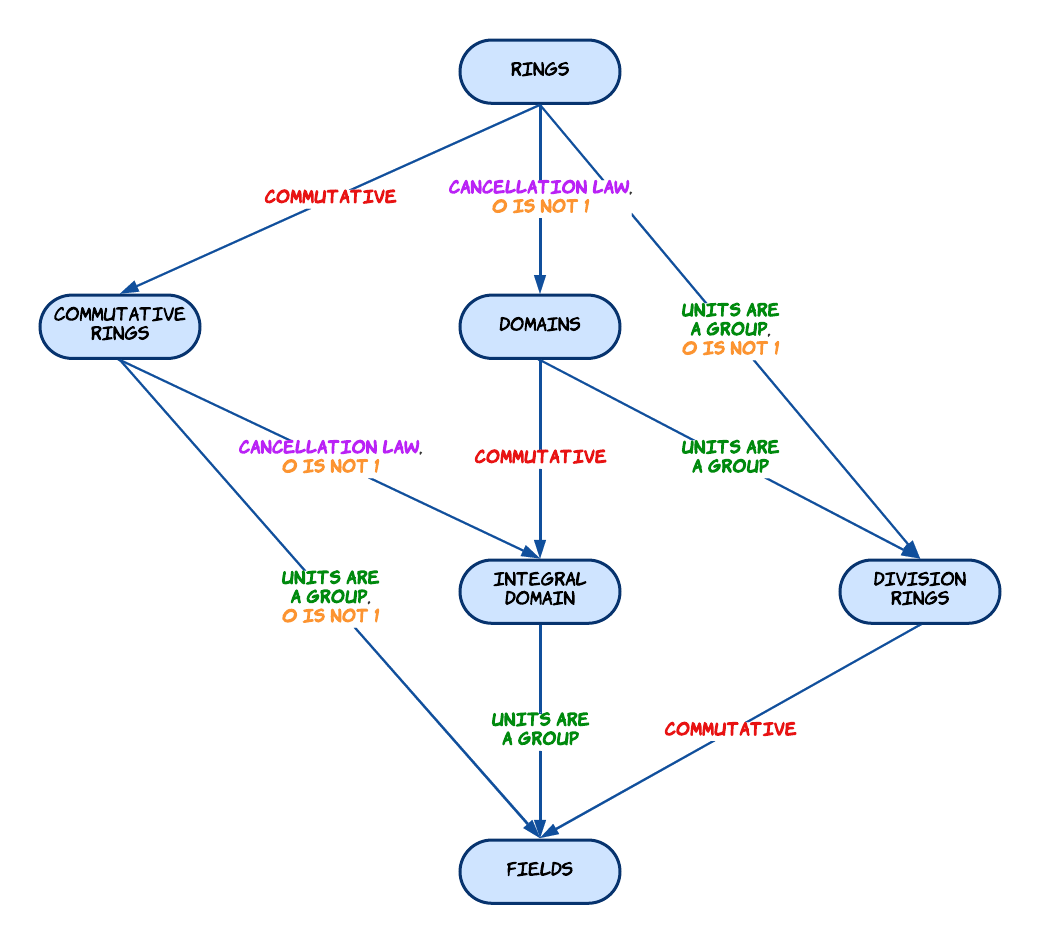
\includegraphics[scale = 0.3]{Ring Diagram}
\centering
\end{figure}

I like that there is a subtle sense of symmetry here. The conditions on the arrow is the condition for the ring in the tail to be a ring in the arrow head. For instance, if a domain $R$ satisfies the property that elements in $R$ are commutative, then $R$ is an integral domain. On the other hand, every integral domain will necessarily be a domain. 

\pagebreak
\subsection{Ring Homomorphisms and Ideals}
\begin{defn}{Ring Homomorphism}{} Let $R,S$ be rings. A ring homomorphism is a map $\phi:R\to S$ such that the following are true: 
\begin{itemize}
\item $\phi(a+b)=\phi(a)+\phi(b)$ for all $a,b\in R$
\item $\phi(ab)=\phi(a)\phi(b)$ for all $a,b\in R$
\end{itemize}
A bijective ring homomorphism is called a ring isomomorphism. 
\end{defn}

\begin{defn}{Left, Right and Two-Sided Ideals}{} Let $(R,+,\cdot)$ be a ring. Let $I\subseteq R$. 
\begin{itemize}
\item $I$ is a left ideal of $R$ if $(I,+)$ is a subgroup of $(R,+)$ and $r\cdot i\in I$ for all $r\in R$ and $i\in I$
\item $I$ is a right ideal of $R$ if $(I,+)$ is a subgroup of $(R,+)$ and $i\cdot r\in I$ for all $r\in R$ and $i\in I$
\item $I$ is a two-sided ideal of $R$ is $I$ is both a left ideal and a right ideal
\end{itemize}
\end{defn}

\begin{lmm}{}{} Let $R$ be a ring. Let $I$ be an ideal of $R$. Then $I=R$ if and only if $I$ contains a unit of $R$. \tcbline
\begin{proof}
Let $I=R$. Then trivially $1\in I$. Now let $u\in I$ be a unit. Let $x\in R$, I want to show that $x\in I$ thus completing the proof that $R\subseteq I$. Now $x=x(u^{-1}u)=(xu^{-1})u$. Since $xu^{-1}\in R$ and $u\in I$, their multiplication will also be in $I$, thus $x\in I$. 
\end{proof}
\end{lmm}

This lemma is also very useful if you consider the fact that the multiplicative identity is also a unit. 

\begin{defn}{Operations on Ideals}{} Let $R$ be a ring. Let $I,J$ be ideals of $R$. 
\begin{itemize}
\item Define the sum of $I$ and $J$ by $$I+J=\{i+j|i\in I,j\in J\}$$
\item Define the intersection of $I$ and $J$ by $$I\cap J=\{r\in R|r\in I,r\in J\}$$
\end{itemize}
\end{defn}

\begin{prp}{}{} Let $R$ be a ring. Let $I,J$ be ideals of $R$. Then $I+J$ and $I\cap J$ are both ideals of $R$. \tcbline
\begin{proof}
Let $R$ be a ring and $I,J$ its ideals. 
\begin{itemize}
\item We first show that $I+J$ is an ideal. Let $i_1+j_1,i_2+j_2\in I+J$. Then since $R$ is an abelian group an $I,J$ are subgroups of $R$, $$i_1+j_1+i_2+j_2=(i_1+i_2)+(j_1+j_2)\in I+J$$ thus closure is satisfied. Associativity is satisfied since it inherits from $R$. We also have $0\in I,J$ thus $0\in I+J$. The inverse of $i+j\in I+J$ is $-i-j\in I+J$ since $-i\in I$ and $-j\in J$. Thus $I+J$ is a subgroup of $R$. \\~\\
Now let $r\in R$ and $i+j\in I+J$. Then $r(i+j)=ri+rj$ by distributivity. Since $I,J$ are ideals, there exists $s\in I$ such that $s=ri$ and $t\in J$ such that $t=rj$. Then $r(i+j)=ri+rj=s+t\in I+J$ thus we are done. 
\item $I\cap J$ are already subgroups of $R$. Let $k\in I\cap J$. Let $r\in R$. Then $rk\in r(I\cap J)$. Then there exists $i\in I$ and $j\in J$ such that $i=rk=j$. Then $i=j\in I\cap J$ thus we are done. 
\end{itemize}
\end{proof}
\end{prp}

\subsection{Types of Ideals}
\begin{lmm}{}{} Let $R$ be a commutative ring and $a\in R$. Then $(a)=\{ar:r\in R\}$ is an ideal. \tcbline
\begin{proof}
Let $s,t\in(a)$. Then $s=ar_1$ and $t=ar_2$ for some $r_1,r_2\in R$. We show that $(a)$ is a subgroup of $R$. We have $$s+t=a(r_1+r_2)\in(a)$$ Identity is also in $(a)$ since $0\in R$ and $$a\cdot 0=0\in(a)$$ To show inverse we have that $u=-ar_1$ and $$s+u=ar_1-ar_1=0$$ By the subgroup criterion, $(a)$ is a group. We now show that $r(a)\subseteq(a)$. Let $r_1ar_2\in r(a)$. Then $$r_1ar_2=ar_1r_2\in(a)$$ since $R$ is commutative. Thus $(a)$ is an ideal. 
\end{proof}
\end{lmm}

\begin{defn}{Principal Ideals}{} Let $R$ be a commutative ring with identity. Let $I$ be an ideal of $R$. Then an ideal $I$ of the form $$I=(a)$$ for some $a\in I$ is called a principal ideal. 
\end{defn}

\begin{defn}{Maximal Ideals}{} A proper ideal $M$ of a ring $R$ is a maximal ideal of $R$ is the ideal $M$ is not a proper subset of any ideal of $R$ except $R$ itself. 
\end{defn}

Becareful that maximal ideals are not necessarily unique. A typical example would be the fact that $(2)$ and $(3)$ are principle ideals that are both maximal in $\Z$. 

\begin{defn}{Prime Ideals}{} A proper ideal $P$ in a commutative ring $R$ is called a prime ideal if $ab\in P$ implies $a\in P$ or $b\in P$. 
\end{defn}

\begin{prp}{}{} Let $R$ be a commutative ring with identity and $M$ an ideal of $R$. Then $M$ is maximal if and only if $R/M$ is a field. \tcbline
\begin{proof}
Suppose that $M$ is a maximal ideal. Let $x\notin R$. We show that $x+M$ has an inverse. We know that $M+(x)$ is an ideal containing $M$. Since $M$ is maximal, we must have $M+(x)=R$. This means that $1\in M+(x)$ which means there exists $m\in M$ and $r\in R$ such that $1=m+rx$. Now consider $r+M$. We have that 
\begin{align*}
(x+M)(r+M)&=xr+M\\
&=(1-m)+M\\
&=1+M
\end{align*}~\\
Now suppose that $R/M$ is a field. Let $J$ be an ideal such that $I\subseteq J\subseteq R$ and $I\neq J$. Now let $x\in J\setminus I$. Then $I+x$ has a multiplicative inverse in $R/I$ since $I+x\neq I$, the additive identity. Let the inverse be $I+y$. Then $$I+1=(I+x)(I+y)=I+xy$$ Trivially $xy\in(x)$, thus $1\in I+(x)\subseteq J$. But if the identity is in the ideal, the ideal is equal to the ring thus we are done. 
\end{proof}
\end{prp}

\begin{prp}{}{} Let $R$ be a commutative ring with identity not equal to $0$. Then $P$ is a prime ideal in $R$ if and only if $R/P$ is an integral domain. \tcbline
\begin{proof}
Suppose that $P$ is a prime ideal. Then let $(a+P)(b+P)=P$. Since we also have that $(a+P)(b+P)=ab+P$. This means that $ab\in P$ thus either $a\in P$ or $b\in P$ which in turns leads to either $a+P=P$ or $b+P=P$ and thus the cancellation law applies. \\~\\
Now suppose that $R/P$ is an integral domain. Let $ab\in P$. Since $R/P$ is an integral domain, we have that $$(a+P)(b+P)=ab+P=P$$ means that either $a+P=P$ or $b+P=P$ which means that either $a\in P$ or $b\in P$ and we are done. 
\end{proof}
\end{prp}

\begin{crl}{}{} Every maximal ideal in a commutative ring with identity is also a prime ideal. \tcbline
\begin{proof}
If $M$ is maximal then $R/M$ being a field implies that $R/M$ is an integral domain thus $M$ is prime. 
\end{proof}
\end{crl}

The proof is rather inconstructive in the sense that it does not provide a good insight to the structure, the reasoning behind why every maximal ideal is prime. For a more structure-revealing proof, consider the following alternative approach: \\~\\
Let $M$ be a maximal ideal of a commutative ring $R$. Let $ab\in M$ but $a\notin M$. Then $M+(a)=R$ since $M$ is maximal. Then $1\in R$ means that there exists $k\in M$ and $r\in R$ such that $k+ra=1$. Mutplying by $b$ gives $kb+rab=b$. Since $kb\in M$ and $rab\in M$, $b\in M$ and we are done. 

\pagebreak
\section{The Isomorphism Theorem for Rings}
\subsection{Kernels and the Quotient Ring}
\begin{defn}{Kernel}{} Let $R,S$ be rings. Let $\phi:R\to S$ be a ring homomorphism. Define the kernel of $\phi$ to be $$\ker(\phi)=\{r\in R\;|\;\phi(r)=0\}$$
\end{defn}

\begin{prp}{}{} Let $R,S$ be a ring. Let $\phi:R\to S$ be a ring homomorphism. Then $\ker(\phi)$ is an ideal of $R$. 
\end{prp}

\begin{prp}{}{} Let $I$ be an ideal of a ring $R$. Then the cosets of $I$ in $R$, $$R/I=\{r+I|r\in R\}$$ is a ring with addition defined the same as quotient groups $$(r+I)+(s+I)=(r+s)+I$$ and multiplication defined as $$(r+I)(s+I)=\{ab\in R|a\in r+I,b\in s+I\}=rs+I$$ \tcbline
\begin{proof}
Since $(I,+)$ is a subgroup of $(R,+)$, we know that $R/I$ is already an abelian group. We simply show that multplication is well defined. Suppose that $x_1+I=x_2+I$ and $y_1+I=y_2+I$. Then 
\begin{align*}
(x_1+I)(y_1+I)&=x_1y_1+I\\
&=(x_1y_1-x_1y_2+x_1y_2-x_2y_2+x_2y_2)+I\\
&=(x_1(y_1-y_2)+(x_1-x_2)y_2+x_2y_2)+I\\
&=x_2y_2+I
\end{align*}
since $y_1-y_2\in I$ and $x_1-x_2\in I$. This shows that taking different represetatives of the cosets of an ideal does not matter for multiplication. \\~\\
Now we show that $1+I$ is the muplicative identity of $R/I$. Let $x+I\in R/I$. We have that $(1+I)(x+I)=x+I$ thus we are done. Associativity and distributivity follows from the fact that $R$ has these properties. 
\end{proof}
\end{prp}

\begin{defn}{Quotient Rings}{} Let $R$ be a ring. Let $I$ be an ideal of $R$. Define the quotient ring of $R$ by $I$ to be the abelian group $$\frac{R}{I}=\{r+I\;|\;r\in R\}$$ together with multiplication defined by $$(r+I)\cdot(s+I)=rs+I$$
\end{defn}

\begin{prp}{}{} Let $R$ be a ring. Let $I\subseteq R$ be a subset. Then $I$ is an ideal of $R$ if and only if it is the kernel of some ring homomorphism. 
\end{prp}

\subsection{Isomophism Theorem for Rings}
The isomorphism theorem for rings is a direct result that extends the group isomorphism theorems. Their proofs are mostly the same except that we also have to check that multiplication is preserved so that the isomorphisms inherited from groups is indeed a ring isomorphism. 

\begin{thm}{The First Isomorphism Theorem for Rings}{} If $\phi:R\to S$ is a homomorphism of rings, then the following are true. 
\begin{itemize}
\item $\ker(\phi)$ is an ideal of $R$
\item $\im(\phi)\leq S$ is a subring of $S$
\end{itemize}
Moreover, we have an isomorphism $$\frac{R}{\ker(\phi)}\cong\phi(R)$$ in rings. \tcbline
\begin{proof}
A group isomorphism $R/\ker(\phi)\cong\phi(R)$ can be established from the first isomorphism theorem for groups. Moreover we know that $\ker(\phi)$ is a normal subgroup. To show that $\ker(\phi)$ is an ideal, notice that for $r\in R$ and $k\in\ker\phi$, $\phi(rk)=\phi(r)\phi(k)=0$ thus $rk\in\ker(\phi)$. To show that $R/\ker(\phi)\cong\phi(R)$ is a ring isomorphism, suppose that $\pi$ is the induced group isomorphism. Notice that 
\begin{align*}
\pi((r_1+\ker(\phi))(r_2+\ker(\phi)))&=\pi(r_1r_2+\ker(\phi))\\
&=\phi(r_1r_2)\\
&=\phi(r_1)\phi(r_2)\\
&=\pi(r_1+\ker(\phi))\pi(r_2+\ker(\phi))
\end{align*}
and so we conclude. 
\end{proof}
\end{thm}

\begin{thm}{The Second Isomorphism Theorem for Rings}{} Let $A\leq R$ and $B$ an ideal of $R$. Then the following are true. 
\begin{itemize}
\item $A+B=\{a+b\;|\;a\in A,b\in B\}$ is a subring of $R$
\item $A\cap B$ is an ideal of $A$
\end{itemize}
Moreover, we have an isomorphism $$\frac{A+B}{B}\cong\frac{A}{A\cap B}$$ in rings. 
\end{thm}

\begin{thm}{The Third Isomorphism Theorem for Rings}{} Let $I,J$ be ideals of $R$ with $I\subset J$. Then $J/I$ is an ideal of $R/I$ and $(R/I)/(J/I)\cong R/J$
\end{thm}

\begin{thm}{The Correspondence Theorem}{} Let $R$ be a ring. Let $I$ be a left ideal of $R$. Then there is an inclusion preserving one-to-one bijection $$\left\{\substack{\text{Subrings of }R\\\text{containing }I}\right\}\;\;\overset{1:1}{\longleftrightarrow}\;\;\left\{\text{Subrings of }R/I\right\}$$ induced by the surjective ring homomorphism $\varphi:R\to R/I$. Moreover, there is an inclusion preserving one-to-one bijection $$\left\{\substack{\text{Ideals of }R\\\text{containing }I}\right\}\;\;\overset{1:1}{\longleftrightarrow}\;\;\left\{\text{Ideals of }R/I\right\}$$ given by the map $A\mapsto A/I$ for $A$ an ideal of $R$ containing $I$. 
\end{thm}

\subsection{Chinese Remainder Theorem}
In this section we develop the necessary notions in order to illustrate the Chinese Remainder Theorem. 

\begin{defn}{Direct product of Rings}{} Let $R,S$ be rings. Define the direct product of $R$ and $S$ to be the set $R\times S=\{(r,s)\in R\times S\}$ together with the binary operations defined element wise. 
\end{defn}

It is a routine exercise to check that $R\times S$ is indeed a ring in its own right. \\~\\

A rather unintuitive definition is that of coprime ideals. 

\begin{defn}{Coprime Ideals}{} We say that two ideals $A,B$ in a ring $R$ are coprime if $A+B=R$. 
\end{defn}

But there is indeed a good reason for the name. Notice that in $\Z$, the prime ideals are exactly the ideals $(p)$ where $p$ is a prime. We also have a nice inclusion of ideals whenever $p|a$ which is $(a)\subseteq(p)$, which we will prove later. This means that in general, the smaller the number $a$ is, the larger the ideal $(a)$ is and indeed, the smaller the number is in $\Z$, the more numbers it can possibly divide. Now recall that if $a$ and $b$ are coprime in $\Z$, then their gcd will be $1$. Indeed we will develop the notion of gcd for ideals as well, which is to say that if $d=\gcd(a,b)$ in the usual sense, then $(a)\subseteq(d)$ and $(b)\subseteq(d)$. Then if $a$ and $b$ are coprime, their ideals are both subsets of $(1)$, which is exactly $R$. This leads to why we say that two ideals are coprime. 

\begin{prp}{}{} Let $A,B$ be ideals of a ring $R$. If $A$ and $B$ are coprime then $$AB=A\cap B$$ \tcbline
\begin{proof}

\end{proof}
\end{prp}

\begin{thm}{Chinese Remainder Theorem}{} Let $I_1,\dots, I_n$ be ideals of a ring $R$. Then the ring homomorphism $$\phi:R\to\frac{R}{I_1}\times\cdots\times\frac{R}{I_n}$$ defined by $\phi(x)=(x+I_1,\dots,x+I_n)$ has kernel $$I=\bigcap_{k=1}^nI_k$$ Moreover, if each $I_j$ and $I_k$ are pairwise coprime, then there is an isomorphism $$\frac{R}{I}\cong\frac{R}{I_1}\times\cdots\times\frac{R}{I_n}$$ given by $\phi$. \tcbline
\begin{proof}
Since $\phi$ is a collection of projections on to each factor, $\phi$ is a ring homomorphism. It is clear that $I$ is the kernel of the homomorphism. Indeed given $x\in I$, then $x$ lies in each and every $I_k$ for $1\leq k\leq n$. Thus $\phi(x)=(x+I_1,\dots,x+I_n)=0$. Conversely, if $(x+I_1,\dots,x+I_n)$ is such that applying $\phi$ gives $0$, then $x\in I_1,\dots,I_n$ so that $x\in I$. \\~\\

When the ideals are pairwise corpime, consider the elements $e_k=(0,\dots,0,x+I_k,0,\dots,0)$ for $1\leq k\leq n$ (these are called full system of orthogonal central idempotents). Notice that they satisfy the equation $1=e_1+\dots+e_n$ and $e_k^2=e_k$ for $1\leq k\leq n$ for $i\neq j$, we have $e_ie_j=0$. Now since $I_i$ and $I_j$ are coprime, we have that $R=I_i+I_j$ so that $1=a_j+z_j$ for $a_j\in I_i$ (note the subscript) and $z_j\in I_j$. Define $x_i=z_1\cdots z_{i-1}\cdot z_{i+1}\cdots z_n$ for each $1\leq i\leq n$. Write the projection homomorphism as $\psi:R\to R/I_j$. If $i\neq j$, then $\phi_j(x_i)=0$ because $x_i$ contains the element $z_j$ that lies in $I_j$. Also, we have that $$\psi_i(z_j)=\psi_i(1-a_j)=\psi_i(1)-\psi_i(a_j)=\psi_i(1)=1$$ in $R/I_i$ since $a_j\in I_i$. Thus we have that $$\psi_i(x_i)=\psi_i(z_1)\cdots\psi_i(z_n)=1$$~\\

All this means that $x_i\in R$ is such that $\psi(x_i)=(0,\dots,0,1+I_i,0,\dots,0)$ for $1\leq i\leq n$. Now to prove surjectivity, let $(r_1,\dots,r_n)$ be an element in the product. Then we have that $$(r_1,\dots,r_n)=\sum_{j=1}^n\psi(r_i)e_i=\sum_{j=1}^n\psi(r_ix_i)$$ and so $r_1x_1+\dots+r_nx_n\in R$ is our desired element. And so we are done. 
\end{proof}
\end{thm}

This is a more generalized version of the Chinese Remainder Theorem in number theory. Indeed, to recover the one in number theory, take $R=\Z$ and $I_k=(n_k)$ for some $n_k\in\Z$ so that $I_k$ is the principal ideal on $n_k$. Moreover, by choosing each $n_k$ to be pairwise coprime, we obtain the isomorphism which proves that the congruence relation can be solved. \\~\\

Notice that the proof is instructive. Indeed we can simply follow the steps of the proof to find a solution. Namely, given $(r_1,\dots,r_n)$ in the product, we can find $r\in R$ such that $\phi(r)=(r_1,\dots,r_n)$. The steps are as follows. 
\begin{enumerate}
\item Fix $1\leq i\leq n$. Using $R=I_i+I_j$, find $a_j\in I_i$ and $z_j\in I_j$ such that $1=a_j+z_j$ for each $j$. This can be done for example by Bezout's lemma in $R=\Z$. 
\item Define $x_i=z_1\cdots z_{i-1}\cdot z_{i+1}\cdots z_n$ for $1\leq k\leq n$. 
\item Do the same for each $1\leq i\leq n$. The solution is then $r=r_1x_1+\dots+r_nx_n$. 
\end{enumerate}


\pagebreak
\section{Integral Domains}
\subsection{Field of Fractions}
\begin{defn}{Fractional Equivalence}{} Let $R$ be an integral domain. Let $$S=\{(a,b)|a,b\in R\text{ and }b\neq 0\}$$ Define a relation on $S$ by $(a,b)\sim(c,d)$ if $ad=bc$. 
\end{defn}

\begin{lmm}{}{} The relation $\sim$ between elements of $S$ is an equivalence relation. \tcbline
\begin{proof}
Since $R$ is an integral domain, symmetry is satisfied. Clearly it is reflexive since $ab=ba$. For transitivity, suppose that $ad=bc$ and $cf=de$. Then $adcf=bcde$ and by cancellation law, $af=be$. 
\end{proof}
\end{lmm}

\begin{prp}{}{} The set of equivalence classes of $S$ of an integral domain $R$, under the equivalence relation $\sim$, together with the operations of addition and multiplication defined by $$(a,b)+(c,d)=(ad+bc,bd)$$ and $$(a,b)\cdot(c,d)=(ac,bd)$$ is a field, called the field of fractions, denoted $\text{Frac}(R)$. \tcbline
\begin{proof} Note that $R$ is a field if and only if $(R,+)$ and $(R\setminus\{0\},\cdot)$ are commutative groups and the distributive law holds. 
\begin{itemize}
\item Let $(a,b),(c,d)\in S$. Then $ad+bc,bd\in R$ since $R$ is closed thus $(ad+bc,bd)\in S$. Let $(e,f)$ also be in $S$. Then 
\begin{align*}
((a,b)+(c,d))+(e,f)&=(ad+bc,bd)+(e,f)\\
&=((ad+bc)f+(bd)e,bdf)\\
&=(adf+bcf+bde,bdf)
\end{align*}
and 
\begin{align*}
(a,b)+((c,d)+(e,f))&=(a,b)+(cf+de,df)\\
&=(a(df)+b(cf+de),b(df))\\
&=(adf+bcf+bde,bdf)
\end{align*}
Thus associativity is satisfied. I claim that $(0,1)$ is an identity. We have $(a,b)+(0,1)(a\cdot 1+b\cdot 0,b\cdot 1)=(a,b)$. If $(a,b)\in S$ then $(-a,b)\sim(a,-b)$ is an inverse. We have $$(a,b)+(-a,b)=(ab-ab,b^2)=(0,b^2)\sim(0,1)$$ Finally we have 
\begin{align*}
(a,b)+(c,d)&=(ad+bc,bd)\\
&=(da+cb,db)\tag{$R$ is an Integral Domain}\\
&=(cb+da,db)\tag{$R$ is an abelian group}
&=(c,d)+(a,b)
\end{align*}
Thus we have shown that $(S,+)$ is an abelian group. 
\item We now show that $(S,\cdot)$ is an abelian group. Let $(a,b),(c,d),(e,f)\in S$. Then $(a,b)\cdot(c,d)=(ac,bd)\in S$ sincve $ac,bd\in R$ by closure of rings. Thus the closure property is satisfied. Associativity is inherited from $R$ since elements in $S$ are pairs of $R$. I claim that the identity is $(1,1)\sim(k,k)$ for any $k\in R$. We have $$(a,b)\cdot(1,1)=(a\cdot1,b\cdot 1)=(a,b)$$ If $(a,b)\in S$ then its inverse is $(b,a)$. We have $$(a,b)\cdot(b,a)=(ab,ba)=(ab,ab)=(1,1)$$ thus $(S,\cdot)$ is a group. Now to show abelian, we have $$(a,b)\cdot(c,d)=(ac,bd)=(ca,db)=(c,d)\cdot(a,b)$$ since $R$ is an integral domain. Thus we have shown that $(S,\cdot)$ is an abelian group. 
\item Finally we show distributivity. Let $(a,b),(c,d),(e,f)\in S$. Then 
\begin{align*}
(a,b)\cdot((c,d)+(e,f))&=(a,b)\cdot(cf+de,df)\\
&=(acf+ade,bdf)
\end{align*}
and 
\begin{align*}
(a,b)\cdot(c,d)+(a,b)\cdot(e,f)&=(ac,bd)+(ae,bf)\\
&=(acbf+bdae,bdbf)\\
&=(acf+ade,bdf)\tag{equivalence relation}
\end{align*}
Thus we are done. 
\end{itemize}
\end{proof}
\end{prp}

In particular, the field of fractions of $\Z$ is precisely $\Q$. 

\begin{lmm}{}{} For any integral domain $R$, $R$ is a subring of $\text{Frac}(R)$. \tcbline
\begin{proof}
Define a function $\phi:R\to Q(R)$ by $\phi(r)=\frac{r}{1}$. Then $\phi_R$ is the identity homorphism thus $\phi(R)=R$. Then $\phi(R)$ is trivially a subring of $Q(R)$ and we are done. 
\end{proof}
\end{lmm}

\subsection{Divisibility}
Division is a property that only commutative rings enjoy. 

\begin{defn}{Division}{} Let $R$ be a commutative ring and let $a,b\in R$ with $b\neq 0$. $a$ is said to be a multiple of $b$ if there exists an element $x\in R$ with $a=bx$. In this case $b$ is said to divide $a$ or be a divisor of $a$, written $b|a$. 
\end{defn}

\begin{prp}{}{} Let $R$ be a commutative ring. Let $x,y\in R$ and $y\neq 0$. Then the following are equivalent. 
\begin{itemize}
\item $x|y$
\item $y\in(x)$
\item $(y)\subseteq(x)$
\end{itemize}\tcbline
\begin{proof} Let $R$ be a commutative ring. Let $x,y\in R$ and $y\neq 0$. 
\begin{itemize}
\item $(1)\implies(2)$ Suppose that $y=kx=xk$ for some $k\in R$. Then $y\in(x)=\{ax|a\in R\}$ by definition. 
\item $(2)\implies(3)$ Suppose that $y\in(x)$. Then there exists $k\in R$ such that $y=kx=xk$. To show that $(y)\subseteq(x)$, let $ry\in(y)$. Then $ry=rkx$ and $rk\in R$ thus $ry\in(x)$ thus we are done. 
\item $(3)\implies(1)$ Suppose that $(y)\subseteq(x)$. Then there exists $k\in R$ such that $y=kx$. Then we are done. 
\end{itemize}
\end{proof}
\end{prp}

\begin{defn}{Greatest Common Divisor}{} Let $R$ be a commutative ring and let $a,b\in R$. A greatest common divisor of $a$ and $b$ is a non-zero element $d\in R$ such that 
\begin{itemize}
\item $d|a$ and $d|b$
\item If $c|a$ and $c|b$ then $c|d$
\end{itemize} It is denoted $\gcd(a,b)$. 
\end{defn}

\begin{defn}{Least Common Multiple}{} Let $R$ be a commutative ring and let $a,b\in R$. A least common multiple of $a$ and $b$ is a non-zero element $l\in R$ such that 
\begin{itemize}
\item $a|l$ and $b|l$
\item If $a|m$ and $b|m$ then $l|m$
\end{itemize} It is denoted $\lcm(a,b)$. 
\end{defn}

Unfortunately, these numbers do not always exists for any $a,b$ in a general ring. The existence of such a number depends on the ideal generated by the two given elements. 

\begin{prp}{}{} Let $R$ be a commutative ring. Let $x,y\in R$ such that they are nonzero. If the ideal generated by $a$ and $b$, namely $(a,b)$ is a principal ideal $(d)$, then $d$ is the gcd of $a$ and $b$. \tcbline
\begin{proof}
Suppose that $(a,b)=(d)$ for some $d\in R$. Then $a\in(d)$ and $b\in(d)$ already implies that $d|a$ and $d|b$. Suppose that $c|a$ and $c|b$. This means that $a\in(c)$ and $b\in(c)$. Since $d\in(a,b)$ there exists $r,s\in R$ such that $ra+sb=d$. This means that $d\in(c)$ thus $c|d$. 
\end{proof}
\end{prp}

\begin{defn}{Associates}{} Let $R$ be a commutative ring. Let $x,y\in R$. We say that $x$ and $y$ are associates if $x|y$ and $y|x$. We denote it as $x\sim y$. 
\end{defn}

\begin{prp}{}{} Let $R$ be a integral domain. Let $x,y\in R$. Then the following are equivalent. 
\begin{itemize}
\item $x\sim y$
\item $(x)=(y)$
\item There exists a unit $u\in R$ such that $x=qy$. 
\end{itemize} \tcbline
\begin{proof}
\begin{itemize}
\item $(1)\implies(2)$: Suppose that $x\sim y$ then $x|y$ and $y|x$ which means that $(x)\subseteq(y)$ and $(y)\subseteq(x)$. 
\item $(2)\implies(3)$: Suppose that $(x)=(y)$. Then since $x\in(y)$, there exists $s\in R$ such that $x=sy$ and likewise $y=tx$. Then $x=stx$ and since $R$ is an integral domain, $st=1$ which means that $s,t$ are units. 
\item $(3)\implies(1)$: Suppose that $x=qy$ for some unit $q$. Then clearly $y|x$. Since $q$ is a unit, $q^{-1}x=y$ and thus $x|y$ which means that $x$ and $y$ are associates. 
\end{itemize}
\end{proof}
\end{prp}

\subsection{Primes and Irreducibles}
Primes and irreducibles are two similar concepts, their difference is only made clear in Euclidean domains that are not principles ideal domains, both of which we will see later. 

\begin{defn}{Irreducibles}{} Let $D$ be an integral domain. A nonzero element $p\in D$ that is not a unit is said to be irreducible if $p=ab$ implies $a$ or $b$ is a unit. 
\end{defn}

\begin{defn}{Primes}{} Let $D$ be an integral domain. A nonzero element $p\in D$ that is not a unit is said to be a prime if $p|ab$ implies $p|a$ or $p|b$. 
\end{defn}

\begin{lmm}{}{} Let $D$ be an integral domain. Let $p$ be a non-unit. Then $p$ is prime if and only if $(p)$ is a prime ideal. \tcbline
\begin{proof}
Suppose that $p$ is prime. Suppose that $rp\in(p)$. Then $p\in P$ and we are done. Now suppose that $(p)$ is a prime ideal. Suppose that $p|ab$. Then $pd=ab$ for some $d\in D$ thus $ab\in(p)$. WLOG take $a\in(p)$ by definition of prime ideal. Then we are done since $a\in(p)$ implies $p|a$. 
\end{proof}
\end{lmm}

\begin{prp}{}{} Let $D$ be an integral domain and $p\in D$. If $p$ is a prime then $p$ is irreducible. \tcbline
\begin{proof}
Let $p$ be a prime in $D$. Suppose that $p=ab$. Then trivially $p|ab$ thus $p|a$ or $p|b$. WLOG take $p|a$. Trivially $a|p$ since $a|ab$. This means that $a$ and $p$ are associates. Thus $p=aq$ for some unit $q$. Then since $aq=ab$ and integral domains have cancellation law, we must have $q=b$ which means that $b$ is a unit. Thus $p$ is irreducible. 
\end{proof}
\end{prp}

\subsection{Unique Factorization Domains}
\begin{defn}{Unique Factorization Domains}{} An integral domain $D$ is a unique factorization domain if the following are true
\begin{itemize}
\item Let $a\in D$ such that $a\neq 0$ and $a$ is not a unit. Then $a$ can be written as the product of irreducible elements in $D$. 
\item Let $a=p_1\cdots p_r=q_1\cdots q_s$, where $p_i$ and $q_j$ are irreducible. Then $r=s$ and there is a permutation such that $p_i=q_{\pi(i)}$ for $i\in\{1,\dots,r\}$. 
\end{itemize}
\end{defn}

Notice that in general integral domains, primes are not the same as irreducibles. But they have the nice property that they coincide in UFDs, which is why they are put in the chapter on UFDs here. Below gives a full converse to the relation between prime and irreducibles we gave above under the umbrealla that is UFDs. 

\begin{prp}{}{} Let $D$ be a UFD and $p\in D$. Then $p$ is a prime if and only if $p$ is irreducible. \tcbline
\begin{proof}
We have already shown the forward implication. Now let $p$ be irreducible. We show that $(p)$ is prime. Let $ab\in(p)$. Then there exists $d\in D$ such that $pd=ab$. We can factorize $ab$ and $pd$ respectively into a product of irreducibles elements in $D$. But since they are equal, by uniqness of fatorization, $p$ is exactly an associate of one of the irreducibles in the factorization of $ab$. If $p$ is in the factorization of $a$ then $p|a$ and we are done. Otherwise it is in $b$ and we are also done. 
\end{proof}
\end{prp}

Notice that in the above proof, the fact that every prime is irreducible does not use the properties of UFD. This means that this is true in general integral domains. 

\subsection{Principal Ideal Domains}
\begin{defn}{Principal Ideal Domains}{} A principal ideal domain is an integral domain in which every ideal is principal, meaning every ideal is of the form $$(a)=\{ra:r\in R\}$$
\end{defn}

\begin{prp}{}{} Let $R$ be a PID and $x,y\in R$. Then $\gcd(x,y)$ and $\lcm(x,y)$ exists and there exists $r,s\in R$ such that $$\gcd(x,y)=rx+sy$$ \tcbline
\begin{proof}
Let $x,y\in R$. Then $(x)+(y)$ is an ideal of $R$, thus it must be prciniple, say $(d)=(x)+(y)$. Similarly, $(x)\cap(y)$ is also an ideal, say $(l)=(x)\cap(y)$. \\~\\
We prove that $d$ and $l$ are the gcd and lcm respectively. Trivially, $(x)\subseteq(d)$ and $(y)\subseteq(d)$ implies $d|x$ and $d|y$. Also for any $z$ such that $z$ divides $x$ and $y$, $(x)\subseteq(z)$ and $(y)\subseteq(z)$ thus $(d)\subseteq(z)$. The proof is similar for $(l)$. \\~\\
Since $(d)=(x)+(y)$, there exists $r,s\in (x),(y)$ respectively such that $d=rx+sy$ and we are done. 
\end{proof}
\end{prp}

\begin{prp}{}{} Let $R$ be a PID and $(p)$ a nonzero ideal in $R$. Then the following are equivalent. 
\begin{itemize}
\item $(p)$ is maximal
\item $p$ is irreducible
\item $p$ is prime ($(p)$ is prime)
\end{itemize} \tcbline
We have seen that every maximal ideal is a prime ideal. We have seen that if $(p)$ is a prime ideal then $p$ is prime. We have also seen that every prime is irreducible. We show separately that if $p$ is irreducible then $p$ is a prime, and also if $p$ is prime then $(p)$ is maximal. \\~\\
For the first part, suppose that $p$ is irreducible. Suppose that $p|ab$ for $a,b\in R$. By the above proposition, $d=\gcd(p,a)$ exists. Then for some $t\in R$, $p=dt$. Since $p$ is irreducible, either $d$ or $t$ is a unit. We consider both cases. If $t$ is a unit, then $p$ and $d$ are associates and thus $p|d$. Since $d|a$, we have that $p|a$ and we are done. Now if $d$ is a unit, then $d=ra+sp$ for some $r,s\in R$. Multplying both sides with $b$ gives $db=rab+spb$. Since $p|ab$ and $p|spb$, we have that $p|db$. Then $pu=db$ for some unit $u\in R$. Since $d$ is a unit, we have that $d^{-1}pu=b$, which means that $p|b$ and we are done. \\~\\
Now we show that if $p$ is a prime then $(p)$ is maximal. We know that $(p)$ is a prime ideal. Suppose that $(p)\subseteq(q)\subseteq R$ for some ideal $q$ of $R$. Since $p\in(q)$, $p=tq$ for some $t\in R$. Since $p\in(p)$, we have that $tq\in(p)$. Now $(p)$ is prime implies that either $t\in(p)$ or $q\in(p)$. If $q\in(p)$ then $(q)\subseteq(p)$ and thus $(q)=(p)$ and we are done. If $t\in(p)$, then $t=rp$ for some $r\in R$, which means that $p=rpq$. Then $rq=1$ by cancallation law in integral domains. This means that $1\in(q)$ thus $(q)=R$ and we are done. 
\end{prp}

\begin{prp}{}{} Every PID is a UFD. \tcbline
\begin{proof}
Suppose that $D$ is a principal ideal domain. Suppose for a contradiction that $x$, a non-unit cannot be factorized into a product of irreducibles. Clearly $x$ is not irreducible else a contradiction. Then there exists $x_1,y_1$ non unit such that $x=x_1y_1$. Since $x$ is assumed to be not a product of irreducibles, WLOG take $x_1$ to be not irreducible. Then we can repeat the process to get non units $x_2y_2$ such that $x_1=x_2y_2$. Notice that $(x)\subset(x_1)$ is a proper containment of ideals if $x_1|x$. Then we have a chain of ideals $$(x)\subset(x_1)\subset(x_2)\subset\dots$$ I claim that $$I=\bigcup_{k=0}^\infty(x_k)$$ is an ideal. Indeed if $r,s\in I$, then $r\in(x_m)$ and $s\in(x_n)$ for some $m,n\in\N$. WLOG rtake $m\leq n$. Then $(x_m)\subseteq(x_n)$ implies $r,s\in(x_n)$ thus $r+s\in(x_n)\subseteq I$. Also if $t\in R$, then $tr\in(x_m)\subseteq I$ thus $I$ is indeed an ideal. \\~\\
Since $R$ is a PID, there exists some $d\in I$ such that $I=(d)$. This also means that $d\in(x_m)$ for some $m\in\N$. Then this means that $I=(d)\subseteq(x_m)$. This proves that the chain eventually stops and this is a contradiction since we assumed that the chain of ideals are properly contained. \\~\\
This menas that $x$ can indeed be factorized into a product of irreducibles. 
\end{proof}
\end{prp}

Notice that the key in the proof is that the union of the countably finite principal ideals is again a principal ideals which allows the infinte chain of ideals to stop. 

\subsection{Euclidean Domains}
Technically, division algorithms can exist in general domains so long that it has the notion of division. But without a measurement of size to guarantee division is taking larger numbers into smaller numbers, we cannot promise that division algorithms will halt eventually. Therefore we restrict the notion of division algorithm only to integral domains that has a notion of size. 

\begin{defn}{Euclidean Valuation}{} Let $R$ be an integral domain. A function $f:R\setminus\{0\}\to\N\cup\{0\}$ is said to be a Euclidean Valuation of $R$ if
\begin{itemize}
\item $f(ab)\geq f(b)$ for all $a,b\in R\setminus\{0\}$
\item For all $a,b\in R$ with $b\neq0$, there exists $q,r$ such that $$a=qb+r$$ with $r=0$ or $f(r)<f(b)$
\end{itemize}
\end{defn}

In the above definition the second item is simply the division algorithm, with size of a number decided by the function $f$. Thus the Euclidean domain is simply an integral domain that possess a division algorithm. 

\begin{defn}{Euclidean Domain}{} An integral domain $R$ is said to be a Euclidean Domain that admits a Euclidean Valuation. 
\end{defn}

\begin{thm}{}{} Let $R$ be a Euclidean Domain. Let $a,b$ be nonzero elements of $R$. Let $d=r_n$ be the last nonzero remainder in the Euclidean Algorithm for $a$ and $b$. Then $d$ is the greatest common divisor of $a$ and $b$ and $(d)$ is generated by $a$ and $b$. In particular, there exists $x,y\in R$ such that $d=ax+by$. 
\end{thm}

\begin{prp}{}{} Every Euclidean Domain is a PID. 
\end{prp}

In general, we have that $$\text{Fields}\subset\text{Euclidean Domains}\subset\text{PID}\subset\text{UFD}\subset\text{Integral Domains}$$ in which all containments are strict. 

\pagebreak
\section{The Ring of Polynomials}
\subsection{Polynomials over General Rings}
In this section we formulate the basic theory of generating polynomials from a ring. 
\begin{defn}{Indeterminates}{} Let $R$ be a ring. A symbol $x$ is called an indeterminate over $R$ if $$a_0+a_1x+a_2x^2+\dots+a_nx^n=0$$ where $a_i\in R$, implies that $a_i=0$ for each $i$. 
\end{defn}

\begin{defn}{Polynomial over a Ring}{} Any expression of the form $$f(x)=\sum_{k=0}^na_kx^k$$ where $x$ is an indeterminate and $a_0,\dots,a_n\in R$ and $a_n\neq 0$ is called a polynomial over $R$. We define the the degree of $f$ in this case to be $n$. 
\end{defn}

\begin{defn}{Ring of Polynomials}{} Let $R$ a ring. Define $R[x]$ to be the set of all polynomials over $R$. 
\end{defn}

\begin{prp}{}{} Let $R$ be a commutative ring with identity. Then $R[x]$ is a commutative ring with identity. \tcbline
\begin{proof}
Since $R\leq R[x]$ by considering all the constant polynomials, the identity of $R$ is also the identity of $R[x]$. Let $f,g\in R[x]$. Then the coefficient of $x^n$ in $f(x)g(x)$ is $$c_n=\sum_{k=0}^na_kb_{n-k}$$ Since $a_kb_{n-k}=b_{n-k}a_k$, we have that $f(x)g(x)=g(x)f(x)$. 
\end{proof}
\end{prp}

\begin{defn}{The Evaluation Map}{} Let $R$ be a ring and let $a$ be an element in the center $Z(R)$ of $R$. Define the evaluation map $\phi_a:R[x]\to R$ by the formula $$\phi_a\left(\sum_{k=0}^nc_kx^k\right)=\sum_{k=0}^nc_ka^k$$
\end{defn}

\begin{thm}{Evaluation Theorem}{} Let $R$ be a ring and let $a$ be an element in the center $Z(R)$ of $R$. Then the evaluation homomorphism $\phi_a:R[x]\to R$ is a surjective ring homomorphism. 
\end{thm}

The evaluation maps gives a useful ring homomorphism to construct quotient rings. 

\begin{lmm}{}{} Let $R$ be a ring. Then the evaluation homomorphism gives an isomorphism $$\frac{R[x]}{(x-a)}\cong R$$ for any $a\in Z(R)$.  \tcbline
\begin{proof}
\end{proof}
\end{lmm}

\subsection{Polynomials over Integral Domains}
\begin{prp}{}{} If $R$ is an integral domain then $R[x]$ is an integral domain. In particular the units in $R$ are also units in $R[x]$. \tcbline
\begin{proof}
Commutativity is clear since for $f,g\in R[x]$, coefficients of the product $fg$ inherits commutativity from $R$ thus $fg=gf$. Now we show that cancellation law exists in $R[X]$. Let $f,g\in R[x]$ such that $fg=0$. Suppose for a contradiction that $f\neq 0$ and $g\neq 0$. This means that $\deg(f)=n$ and $\deg(g)=m$ for some $n,m\neq 0$. Consider the coefficient of $x^{n+m}$ in $fg$, which is $a_nb_m$. Since $fg=0$, $a_nb_m=0$ and by cancellation law in $R$ either $a_n=0$ or $b_m=0$. This contradicts the fact that $\deg(f)=n$ and $\deg(g)=m$ thus we are done. \\~\\
The second part is trivial since $R\leq R[x]$ and they have the same identity. 
\end{proof}
\end{prp}

\begin{prp}{}{} Let $R$ be an integral domain. Then if $f\neq 0$ and $g\neq 0$ in $R[x]$, then $$\deg(fg)=\deg(f)+\deg(g)$$
\end{prp}

\begin{prp}{}{} Let $R$ be a commutative ring. Let $I$ be an ideal of $R$. Then the following are true. 
\begin{itemize}
\item $I[x]$ is an ideal of $R$
\item There is an isomorphism $\frac{R[x]}{I[x]}\cong\frac{R}{I}[x]$ given by the map $\left(f=\sum_{k=0}^na_kx^k+I[x]\right)\mapsto\left(\sum_{k=0}^n(a_k+I)x^k\right)$
\item If $I$ is a prime ideal of $R$, then $I[x]$ is a prime ideal of $R[x]$. 
\end{itemize}
\end{prp}

\subsection{Polynomials over UFDs}
The primary goal of this chapter is to compute results relating to finding out ireducible polynomials in UFD, rather than investigating the structure of polynomial rings. 
\begin{defn}{Primitive}{} An element $0\neq f\in R[x]$ where $R$ is a unique factorization domain is called primitive if $\gcd(a_0,a_1,\dots,a_n)=1$. 
\end{defn}

The reason that we have this notion is to prevent polynomials such as $5x-5$ to be discussed. This clearly will not be irreducible since there is a factor of $5$. Likewise if the gcd of all its coefficients are not $1$, then you can factor out the gcd from the entire polynomial. 

\begin{prp}{}{} The productive of two primitive polynomials is also primitive. 
\end{prp}

\begin{prp}{Eisentein's Criterion}{} Let $R$ be a UFD. Let $f\in R[x]$ be primitive. Suppose there is a prime $p\in R$ such that $p$ does not divide $a_n$ but $p|a_i$ for $0\leq i\leq n-1$ and $p^2$ does not divide $a_0$. Then $f$ is irreducible in $R[x]$. 
\end{prp}

\begin{thm}{}{} Let $R$ be a UFD with field of fractions $Q=Q(R)$. Then a primitive polynomial in $R[x]$ is irreducible if and only if it is irreducible in $Q[x]$. 
\end{thm}

\begin{prp}{}{} $R$ is an UFD if and only if $R[x]$ is an UFD. 
\end{prp}

\subsection{Polynomials over a Field}
This section will mainly be revisiting old notations with $F[x]$. 
\begin{thm}{Division Algorithm}{} Let $F$ be any field and let $f$ and $g$ be polynomials in $F[x]$. Assume that $f\neq0$ and that the leading coefficient of $f$ is a unit in $R$. Then uniquely determined polynomials $q$ and $r$ exist in $F[x]$ such that 
\begin{itemize}
\item $g=qf+r$
\item Either $r=0$ or $\deg(r)<\deg(f)$
\end{itemize}
In particular, $\deg$ is an Euclidean Valuation of $F[x]$ and $F[x]$ is a Euclidean domain. 
\end{thm}

The above theorem is equivalent to saying that $F[x]$ is a Euclidean domain as long as $F$ is a field. Trivially, this also means that $F[x]$ is both a principal ideal domain and a unique factorization domain. \\~\\
We give an alternate proof showing that $F[x]$ is a principal ideal domain. \\~\\
Let $I$ be a nontrivial ideal of $F[x]$. Let $f\in I$ be nonzero such that the degree of $f$ is as small as possible. I claim that $(f)=I$. We already have that $(f)\subseteq I$ since $f\in I$. Now we show that $I\subseteq(f)$. So let $g\in I$. By the division algorithm, write $g=fq+r$ for some $q,r$ such that $\deg(r)<\deg(f)$ or $\deg(r)=0$. If $r\neq 0$, then $r=g-fq\in I$ since $f,g\in I$. But then $\deg(r)<\deg(f)$ means that $f$ is not of smallest degree in $I$, a contradiction. Thus $g=fq$, which means that $g\in(f)$. \\~\\
This is a constructive proof in the sense that if we would like to know the sole generator of an ideal in a polynomial ring $F[x]$ of a field, we simply take the polynomial of lowest degree. \\~\\

Since we have shown that polynomials over a field are euclidean domains, the following theorems and definitions are also trivial. 

\begin{lmm}{}{} Let $F$ be a field and suppose that $p\in F[x]$. Then the ideal generated by $p$ is maximal if and only if $p$ is irreducible. \tcbline
\begin{proof}
Proved when we introduced irreducibility. 
\end{proof}
\end{lmm}

\begin{prp}{Greatest Common Divisor}{} Let $f$ and $g$ be nonzero polynomials in $F[x]$, where $F$ is a field. Then a uniquely determined polynomial $d$ exists in $F[x]$ satisfying the following conditions. 
\begin{itemize}
\item $d$ is monic
\item $d$ divides both $f$ and $g$
\item If $h$ divides both $f$ and $g$, then $h$ divides $d$
\item $d=uf+vg$ for some polynomials $u,v\in F[x]$
\end{itemize}
\end{prp}

\begin{prp}{}{} Let $p\in F[x]$ be irreducible, $F$ a field. If $p$ divides a product $f_1f_2\cdots f_n$ of nonzero polynomials in $F[x]$, then $p$ divides one of $f_i$. 
\end{prp}

\begin{thm}{Unique Factorization Theorem}{} If $F$ is a field, let $f$ be a nonconstant polynomial in $F[x]$. Then 
\begin{itemize}
\item $f=ap_1p_2\cdots p_n$, where $a\in F$ and $p_i$ is monic and irreducible for all $i$
\item The factorization is unique up to the order of the factors
\end{itemize}
\end{thm}

We now begin dicussion of new notions that only polynomial rings based on a field will have. 

\begin{thm}{Factor Theorem}{} Let $F$ be a field. Let $a\in R$. Let $f\in F[x]$. Then $f(a)=0$ if and only if $f=(x-a)q$ for some $q\in F[x]$. \tcbline
\begin{proof}
Clearly if $f$ is of the form $f=(x-a)q$ then $f(a)=0$. \\~\\
Now suppose that $f(a)=0$. We apply the division algorithm on $f$ with $x-a$ to get $$f(x)=(x-a)q(x)+r(x)$$ where either $r(x)=0$ or $\deg(r)<1$. This means that $r(x)=k$ for some constant $k\in F$. Since $f(a)=0$, we have that $(a-a)q(a)+k=0$ which means that $k=0$ and we are done. 
\end{proof}
\end{thm}

\begin{prp}{}{} Let $F$ be a field and let $f$ be a nonzero polynomial in $F[x]$ of degree $n$. Then $f$ has at most $n$ roots in $R$. 
\end{prp}

\begin{thm}{Remainder Theorem}{} Let $F$ be a field. Let $a\in F$. Let $f\in F[x]$. If $f$ is divided by $(x-a)$, the remainder is $f(a)$. \tcbline
\begin{proof}
By division algorithm, there exists $q,r\in F[x]$ such that $f(x)=(x-a)q(x)+r(x)$. Evaluating $x$ at $a$ gives $f(a)=r(a)$. 
\end{proof}
\end{thm}

\subsection{Factorization in $\Z[x]$ and $\Q[x]$}
Gauss's lemma reduces the question of irreducibility in $\Q[x]$ half to $\Z[x]$. 

\begin{thm}{Gauss's Lemma}{} A primitive irreducible polynomial in $\Z[x]$ remains irreducible in $\Q[x]$
\end{thm}

Eisenstein's criterion is particularly useful in $\Z[x]$. 

\begin{thm}{Eisensteins's Criterion}{} Let $f(x)=\sum_{k=0}^na_kx^k\in\Z[x]$. Suppose that $p$ is a prime such that 
\begin{itemize}
\item $p$ does not divide $a_n$
\item $p$ divides $a_0,\dots,a_{n-1}$
\item $p^2$ divides $a_0$
\end{itemize}
Then $f$ is irreducible in $\Z[x]$. 
\end{thm}

The rational root test shows that any rational number that is a root of $f$ must satisfy divisibility criterion, which reduces the number of rationals that we have to check for roots. 

\begin{thm}{Rational Root Test}{} Let $f(x)=\sum_{k=0}^na_kx^k\in\Z[x]$. If $r/s\in\Q$ for $\gcd(r,s)=1$ is a root then $r$ divides $a_0$ and $s$ divides $a_n$. 
\end{thm}

Finally, recall that $\F_p\cong\Z/p\Z$ is a field. We can descend the polynomial to the prime field and check irreducibility there. This is typically easier for small primes since there are less total roots to check in that case. 

\begin{thm}{}{} Let $f(x)=\sum_{k=0}^na_kx^k\in\Z[x]$. Suppose that $p$ is a prime such that $p$ does not divide $a_n$. Write $\overline{a_k}\equiv a_k\;(\bmod\;p)$ for $0\leq k\leq n$ and $$\overline{f}=\sum_{k=0}^n\overline{a_k}x^k\in\F_p[x]$$ If $\overline{f}$ is irreducible in $\F_p[x]$ then $f$ is irreducible in $\Z[x]$. 
\end{thm}


\pagebreak

\section{Field Theory}
\subsection{Properties of a Field}
\begin{defn}{Fields}{} A field is a commutative division ring, denoted $(F,+,\times)$. In particular, it satisfies the following
\begin{itemize}
\item $(F,+)$ is an abelian group with identity $0$
\item $(F\setminus\{0\},\times)$ is an abelian group with identity $1$
\item (Distributivity) $a(b+c)=ab+ac$ for $a,b,c\in F$
\end{itemize}
\end{defn}

\begin{defn}{Subfields}{} A subfield is a subset $E$ of a field $F$ such that the subset is a field. It is denoted $E<F$
\end{defn}

\begin{prp}{}{} A commutative ring is a field if and only if its only ideals are the trivial ideal and the ring itself. \tcbline
\begin{proof}
Let $F$ be a field. Suppose that $I$ is a non trivial ideal of $F$. Then there exists $i\in I$. Since $I$ is an ideal, then $i^{-1}I\subseteq I$ thus $i^{-1}i=1\in I$. But $1$ in $I$ implies that $I=F$ thus we are done. \\~\\
Suppose that the non trivial ideal of a commutative ring $R$ is only $R$ itself. We want to show that every element except $0$ is a unit. Let $r\in R\setminus\{0\}$. Then the principal ideal $(r)$ is nonzero and thus $(r)=R$. Then there exists $b\in R$ such that $rb=br=1$. Thus $b$ is an inverse of $r$. 
\end{proof}
\end{prp}

\begin{prp}{Characteristic}{} Let $F$ be a field. Then either $\text{char}(F)=0$ or $\text{char}(F)=p$ a prime number. \tcbline
\begin{proof}
Suppose that $\text{char}(F)=a\cdot b\neq 0$. Then $(a\cdot b)\cdot 1=0$ implies that $a=0$ or $b=0$ since $F$ is an integral domain. Either way this implies $\text{char}(F)=0$ which is a contradiction. 
\end{proof}
\end{prp}

As usual in understanding different structures in algebra, it is important to study the homomorphisms betweens the structure. 

\begin{defn}{Field Homomorphisms}{} Let $F,K$ be fields. A field homomorphism from $F$ to $K$ is a ring homomorphism $\phi:F\to K$. 
\end{defn}

The structure of fields are very rich and thus they are very rigid. 

\begin{lmm}{}{} Let $F,K$ be fields and $\phi:F\to K$ a field homomorphism. Then $\phi$ is injective. \tcbline
\begin{proof}
Suppose that $a\in\ker(\phi)$. Then we have $\phi(a)\phi(a^{-1})=\phi(aa^{-1})=1$ and $\phi(a)\phi(a^{-1})=0$. Thus there is a contradiction. 
\end{proof}
\end{lmm}

In particular, a field homomorphism $\varphi:F\to K$ means that $F$ embeds into $K$ since $F$ is now isomorphic to $\varphi(F)$ which is a subfield of $K$. Instead of writing $\varphi(F)$ a subfield of $K$ we will write $F\subset K$ instead. This embedding however depends on $\varphi$ and so the embedding is unclear, we will use $\varphi(F)\subset K$ for $F$ being isomorphic to a subfield of $K$. 

\subsection{Types of Fields}
\begin{defn}{Prime Subfields}{} Let $F$ be a field. The prime subfield of $F$ is the subfield of $F$ generated by the multiplicative identity of $F$. Namely the field $\{n\cdot 1|n\in\Z\}$. 
\end{defn}

\begin{prp}{}{} Let $F$ be a field. The prime subfield is equal to $$\bigcap_{K<F}K$$ \tcbline
\begin{proof}
The fact that it is a field itself is trivial. Write $E$ for the prime subfield. Let $L=\bigcap_{K<F}K$.  Then $L<E$ is trivial. Now $1\in L$ since $L$ is a subfield of $F$. Since $E$ is the smallest subfield containing $1$, $E<L$ and we are done. 
\end{proof}
\end{prp}

\begin{prp}{}{} The prime subfield of a field $F$ is isomorphic to either $\Q$ or $\Z/p\Z$
\end{prp}

\begin{defn}{Composite Field}{} Let $E,F<K$. Then the composite field $FE$ is defined to be the smallest subfield of $K$ that contains both $E$ and $F$. 
\end{defn}

\begin{prp}{}{} Let $E,F<K$. Then $$FE=\bigcap_{\substack{U\text{ a field}\\E,F<U<K}}U$$
\end{prp}

\subsection{Field Extensions}
\begin{defn}{Field Extensions}{} Let $F,K$ be fields such that $K$ contains $F$ as a subfield. Then we say that $K$ is a field extension of $F$ and we write it as $F<K$. \\~\\
If $F<L<K$ are field extensions then we say that $L$ is the intermediate field of the extension $F<K$. 
\end{defn}

\begin{prp}{}{} If $K$ is an extension of $F$, then $K$ is a vector space over $F$. \tcbline
\begin{proof}
Define the action of $F$ on $K$ by simply left multiplication. Then the axioms of a vector space is satisfied through properties of $F$ as a field. 
\end{proof}
\end{prp}

\begin{defn}{Degree of an Extension}{} Let $K/F$ be a field extension. The degree of $K/F$, denoted $$[K:F]$$ is the dimension of $K$ as a vector space over $F$. It is said to be finite if $[K:F]$ is finite and infinite otherwise. 
\end{defn}

\begin{prp}{The Tower Law}{} Let $F<K<E$ be field extensions. Then $$[E:F]=[E:K][K:F]$$ Moreover, if $\{a_i|i\in I\}$ is a basis for $E$ over $K$ and $\{b_j|j\in J\}$ is a basis for $K$ over $F$ then $$\{a_ib_j|i\in I, j\in J\}$$ is a basis for $E$ over $F$. 
\end{prp}

\begin{defn}{Finite Extensions}{} Let $K/F$ be a field extension. We say that $K/F$ is a finite extension if $[K:F]$ is finite. 
\end{defn}

\subsection{Finitely Generated Field Extensions}
Recall the evaluation map $\phi_a:F[x]\to K$ given by $f\mapsto f(a)$ for each $a\in K$. 

\begin{defn}{Simple Extensions}{} Let $F<K$ be a field extension. Let $a\in K$. Define 
$$F(a)=\left\{\frac{\phi_a(f(x))}{\phi_a(g(x))}\bigg{|}f,g\in F[x],g(a)\neq 0\right\}=\left\{\frac{f(a)}{g(a)}\bigg{|}f,g\in F[x],g(a)\neq 0\right\}$$
We say that a field extension $F<L$ is a simple extension if $L=F(a)$ for some $a\in L$. 
\end{defn}

It is straight forward from the definition to see that $F(a)$ is just the fraction field of $F[a]$. 

\begin{lmm}{}{} Let $K/F$ be a field extension. Let $a\in K$. Then $$\text{Frac}(F[a])=F(a)$$
\end{lmm}

\begin{prp}{}{} Let $F<K$ be a field extension. Then $K=F(a)$ is a simple field extension for $a\in K$ if and only if $$K=\bigcap_{\substack{R\text{ is a field}\\F\cup\{a\}\subseteq R\subseteq K}}R$$
\end{prp}

Similar to simplex extensions, we can adjoin multiple elements to a field. 

\begin{defn}{Finitely Generated Field Extensions}{} Let $K/F$ be a field extension. Let $\{a_1,\dots,a_n\}\subset K$. Define $$F(a_1,\dots,a_n)=\left\{\frac{\phi_a(f(a_1,\dots,a_n))}{\phi_a(g(a_1,\dots,a_n))}\;\bigg{|}\;f,g\in F[x_1,\dots,x_n],g(a_1,\dots,a_n)\neq 0\right\}$$ to be the field extension finitely generated by $a_1,\dots,a_n$. 
\end{defn}

In particular, finitely generated extensions is just the simple extension applied finitely many times. 

\begin{lmm}{}{} Let $F<K$ be fields. Let $a,b\in K$, then $F(a,b)=F(a)(b)$. 
\end{lmm}

\begin{prp}{}{} Let $K/F$ be a field extension. Let $X=\{a_1,\dots,a_n\}\subset K$. Then $$F(a_1,\dots,a_n)=\bigcap_{\substack{R\text{ is a field}\\F\cup X\subseteq R\subseteq K}}R$$ Namely, it is the smallest field extension of $F$ containing $X$. 
\end{prp}

\begin{prp}{}{} Every finite field extension is finitely generated. \tcbline
\begin{proof}
Let $K/F$ be a finite field extension, say $n=[K:F]$. Then by definition, $K=\text{span}\{k_1,\dots,k_n\}$ where $k_i\in K$ for each $i$. Hence every element of $K$ can be written as a finite linear combination of $k_1,\dots,k_n$ over $F$. Thus $K\subseteq F(x_1,\dots,x_n)$. Since $K$ is a field that contains $F$ and $\{k_1,\dots,k_n\}$, by proposition 9.4.6, we have that $F(k_1,\dots,k_n)\subseteq K$ and so we conclude. 
\end{proof}
\end{prp}

There is a great relation between the polynomial ring and finitely generated field extensions. Notice that a polynomial ring over a field is not a field while finitely generated field extensions are a field. 

\begin{prp}{}{} Let $K/F$ be a field extension. Let $X=\{a_1,\dots,a_n\}\subset K$. Then $$F[a_1,\dots,a_n]=\bigcap_{\substack{R\text{ is a ring}\\F\cup X\subseteq R\subseteq K}}R$$
\end{prp}

\begin{prp}{}{} Let $K/F$ be a field extension. Let $X=\{a_1,\dots,a_n\}\subset K$. Then $$F(a_1,\dots,a_n)=\text{Frac}\left(F[a_1,\dots,a_n]\right)$$
\end{prp}

\subsection{Algebraic Elements}
Recall the notion of algebraic elements and the minimal polynomials from groups and rings. 

\begin{defn}{Algebraic and Transcendental Elements}{} Let $F<K$ be fields. Then $a\in K$ is said to be algebraic over $F$ if there exists a non zero polynomial $f\in F[x]$ such that $f(a)=0$. Otherwise it is said to be transcendental. 
\end{defn}

\begin{defn}{Minimal Polynomial}{} Let $F<K$ be field extensions and $a\in K$ be algebraic over $F$. Then the minimal polynomial of $a$ over $F$ is the monic irreducible polynomial $p(x)\in F[x]$ of least degree such that $p(a)=0$. It is often denoted $\min(F,a)$. 
\end{defn}

\begin{prp}{}{} Let $F<K$ be fields and $a\in K$ be algebraic over $F$. Then the minimal polynomial exists and is unique. Moreover, if $g\in F[x]$ satisfies $g(a)=0$, then $f|g$. 
\end{prp}

\begin{prp}{}{} Let $F<K$ be a field extension and $a\in K$ algebraic over $F$. Let $\deg(\min(F,a))=n$. Then $[F(a):F]=n$ and $1,a,\dots,a^{n-1}$ is a basis for $F(a)$ over $F$. \tcbline
\begin{proof}
Suppose that $f$ is the minimum polynomial. We prove that $L:F[x]_{<n}\to F[x]/(f)$ defined by $L(g)=g+(f)$ is a field isomorphism. It is easy to check that it is a $F$-linear map. For injectivity, suppose that $L(v)=0$. Then $v\in(f)$ as well as $\deg(v)<\deg(f)$ by construction forces $v$ to be $0$. For sujectivity, suppose that $r+(f)\in F[x]/(f)$ and $\deg(r)<\deg(f)$. Then we can just choose $r\in F[x]_{<n}$ and we are done. Thus $L$ is an isomorphism. \\~\\
Using the fact that $F[x]/(f)\cong F(a)$, we can construct a basis for $F(a)$ from $L$. But $L$ has the basis $\{1,x,\dots,x^{n-1}\}$. Transporting it through the field isomorphisms, we get $\{1,a,\dots,a^{n-1}\}$ is a basis of $F(a)$. \\~\\
\end{proof}
\end{prp}

\begin{prp}{}{} Let $f\in K[x]$ be an irreducible polynomial. Then there exists a field extension $K<L$ and $a\in L$ such that $L=K(a)$ and $f(a)=0$. \\~\\

Moreover, if $f$ is monic, then $f$ is the minimal polynomial of $a$ over $K$ and $[K(a):K]=\deg(f)$. \tcbline
\begin{proof}
Consider the field $L=K[x]/(f)$. $L$ is a field since $f$ is irreducible in $K[x]$. Moreover, the composition $K\to K[x]\to K[x]/(f)=L$ is a field homomorphism and so is injective. Let $a=x+(f)\in L$. Any element of $L$ is of the form $h(x)+(f)$, but that is exactly $h(a)$, so $a$ generates $L$ over $K$. It is clear that $f(a)=f(x)+(f)=0+(f)$ is zero in $L$. \\~\\

If $f$ is monic and irreducible, it is by definition the minimal polynomial of $a$. By the above theorem, $[K(a):K]=\deg(f)$ and so we conclude. 
\end{proof}
\end{prp}

If $f$ is reducible, then we will not have the last statement that $[K(a):K]=\deg(f)$, but the rest of the proposition still works, just pick your favourite irreducible factor of $f$. 

\subsection{Algebraic Extensions}
Every field extension can be classified into an algebraic extension or a transcendental extension or a mixture of both. Since $\R$ contains both algebraic elements and transcendental elements of $\Q$, it is the prototypical example of such a field extension. Algebraic extensions will be studied briefly here, while more is said on transcendental extensions in field and Galois theory. 

\begin{defn}{Algebraic Extensions}{} Let $K/F$ be a field extension. We say that $K/F$ is an algebraic extension if every element of $K$ is algebraic over $F$. 
\end{defn}

In particular, notice that $a\in K$ is an algebraic element over $F$ if and only if $F(a)$ is an algebraic extension. 

\begin{lmm}{}{} If $F<K$ is a finite extension of fields, then $K$ is algebraic over $F$. \tcbline
\begin{proof}
Suppose that $[K:F]=n$. If $a\in L$, consider the elements $1,a,\dots,a^n$. Since they lie in an $n$ dimensional vector space, there exists $c_0,\dots,c_n\in F$ not all $0$ such that $\sum_{i=0}^nc_ia^i=0$. Thus $a$ satisfies a non-trivial polynomial relation over $F$. 
\end{proof}
\end{lmm}

\begin{thm}{}{} If $K$ is algebraic over $L$ and $L$ is algebraic over $F$ then $K$ is algebraic over $F$. 
\end{thm}

\begin{prp}{}{} Let $K$ be a field extension of $F$. If each $a_1,\dots,a_n\in K$ is algebraic over $F$, then $F(a_1,\dots,a_n)$ is a finite dimensional vector space with $$[F(a_1,\dots,a_n):F]\leq\prod_{k=1}^n[F(a_k):F]$$
\end{prp}

\begin{crl}{}{} Let $F<K$ be fields. Then $a\in K$ is algebraic over $F$ if and only if $[F(a):F]<\infty$. \\~\\

Moreover, a simple field extension $F(a)/F$ is a finite extension if and only if $F(a)$ is an algebraic extension. 
\end{crl}

Since finitely generated field extensions is a finite concatenation of simple extensions, we can ask the question of whether the simplicity criteria can be relaxed to finitely generated extensions. The following proposition shows that it is possible. 

\begin{prp}{}{} Let $K/F$ be a finitely generated field extension. Then $K/F$ is a finite extension if and only if $K/F$ is an algebraic extension. 
\end{prp}

If one know of colimits, then it is easy to see that algebraic extension are just colimits of finite extensions. This means that algebraic extensions are just finite extensions applied a countable number of times. 

\end{document}